% main.tex

\section{Perturbative results}
\label{sec:integrability}

\begin{chapquote}{Old Chinese Proverb}
It is better to take many small steps in the right direction than to make a great leap forward only to stumble backward.
\end{chapquote}

\noindent In this section we start attacking the problem of finding the spectrum and as expected we begin with perturbation theory.
Starting at weak coupling we quickly stumble upon an amazing feature of the theory, so-called integrability, which allows one to apply numerous techniques that greatly simplify the problem.
We demonstrate integrability from the string theoretic perspective at strong coupling as well, which suggests a unified picture of the integrable structure embedded in the theory persisting to all loops.
After discussing results achievable via integrability in the perturbative regime we finish off with our first exact result, the slope function, which in turn allows one to extract novel information about the spectrum.

\subsection{One loop at weak coupling}
\label{sec:integrability_weak}

We begin with two point correlation functions of local operators.
In any conformal field theory they are constrained by symmetry, namely for operators that are eigenvalues of dilatations they have the following form at all loop levels
\begin{equation}
	\left< \mathcal{O}(x) \, \tilde{\mathcal{O}}(y) \right> \approx \frac{1}{|x-y|^{2\Delta}},
\end{equation}
where $\Delta$ is the scaling dimension of the operator and we ignore unphysical normalization factors. 
Classically $\Delta = \Delta_0$ is simply the mass dimension, but at the quantum level it receives radiative corrections and acquires an anomalous dimension $\gamma$, such that $\Delta(g_{YM}) = \Delta_0 + \gamma(g_{YM})$, where the anomalous dimension depends on the coupling. 
Usually the corrections are small and the correlator can be expanded perturbatively.
Of course one has to be careful here, as expanding in $\gamma$ would result in expressions like $\log|x-y|$, which do not make sense. 
To that end we introduce a scale $\mu$ and expand the following quantity instead 
\begin{equation}
	\mu^{-2\gamma} \left< \mathcal{O}(x) \, \tilde{\mathcal{O}}(y) \right> \approx \frac{1}{|x-y|^{2\Delta_0}} \left(1 - \gamma \log \mu^2 |x-y|^2 \right),
	\label{eq:anomdim_expansion}
\end{equation}
however we will formally assume that the factor $\mu^{-\gamma}$ is absorbed into the field definition and thus we will ignore it from now on. We can now take some explicit local operator $\mathcal{O}(x)$, calculate the correlator using perturbation theory and read off the anomalous dimension $\gamma$.
Let us start with a very simple chiral primary operator 
\begin{equation}
	\Psi = \tr \, Z^L  = {Z^a}_b {Z^b}_c \dots {Z^l}_a,
	\label{eq:primary_op}
\end{equation}
where the complex scalar field $Z$ and its conjugate $\tilde{Z}$ have the standard tree level correlators
\begin{equation}
	\left< {Z^a}_b(x) {{\tilde{Z^{b'}}}}_{a'}(y) \right>_{\mathrm{tree}} \approx \frac{{\delta^a}_{a'} {\delta_b}^{b'}}{|x-y|^{2}}.
	\label{eq:z_correlator}
\end{equation}  
In order to find the anomalous dimension of the operator $\Psi$ we must calculate the correlator $\langle\Psi(x) \tilde{\Psi}(x)\rangle$. We do this by using Wick's theorem and plugging in the two-point correlator (\ref{eq:z_correlator}), which produces a lot of terms with delta function contractions between the adjoint indices. Some examples are
\begin{subequations}
	\begin{equation} 
	\dots {\delta^{a'}}_{a} \; {\delta^{a}}_{a'} \; {\delta^{b'}}_{b} \; {\delta^{b}}_{b'} \; {\delta^{c'}}_{c} \;  {\delta^{c}}_{c'} \; \dots 
	\end{equation}
	\vspace{-22pt}
	\begin{equation}
	\dots {\delta^{a'}}_{c} \; {\delta^{c}}_{a'} \; {\delta^{b'}}_{a} \; {\delta^{a}}_{b'} \; {\delta^{c'}}_{b} \;  {\delta^{b}}_{c'} \; \dots 
	\end{equation}
	\begin{equation}
	\dots {\delta^{a'}}_{a} \; {\delta^{a}}_{b'} \; {\delta^{c'}}_{b} \; {\delta^{b}}_{a'} \; {\delta^{b'}}_{c} \;  {\delta^{c}}_{c'} \; \dots 
	\end{equation}
	\label{eq:delta_contractions}
\end{subequations}
\begin{figure}[t]
\centering
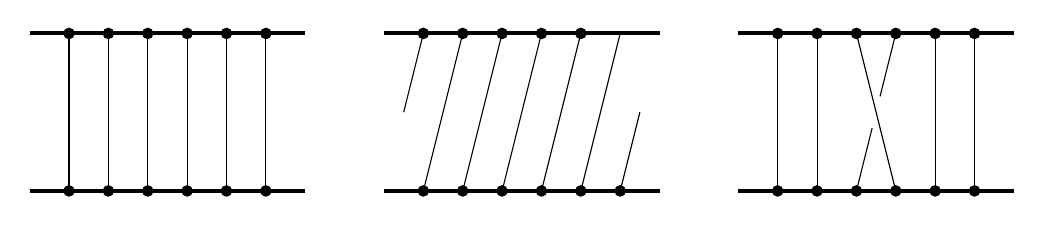
\begin{tikzpicture}[scale=0.5,every node/.style={draw,shape=circle,fill=black,scale=0.4}]
	
	%\draw[help lines] (0,0) grid (29,5);

	\def\height{4}
	\def\width{7}
	\def\gap{2}
	
	\begin{scope}[shift={(\gap,0)}]
	
		\draw[line width=0.5mm] (0,0) -- (\width,0);
		\draw[line width=0.5mm] (0,\height) -- (\width,\height);
		
		\foreach \x in {1,2,3,4,5,6} {
			\node at (\x, 0) {}; \node at (\x, \height) {};
			\draw (\x,0) -- (\x,\height);
		}

	\end{scope}
	
	\begin{scope}[shift={(\width+2*\gap,0)}]
	
		\draw[line width=0.5mm] (0,0) -- (\width,0);
		\draw[line width=0.5mm] (0,\height) -- (\width,\height);
		
		\foreach \x in {1,2,3,4,5} {
			\node at (\x, 0) {}; \node at (\x, \height) {};
			\draw (\x,0) -- (\x+1,\height);
		}
		
		\node at (6, 0) {}; ;
		
		\draw (0.5, \height / 2) -- (1,\height);
		\draw (6,0) -- (6.5,\height / 2);

	\end{scope}
	
	\begin{scope}[shift={(2*\width+3*\gap,0)}]
	
		\draw[line width=0.5mm] (0,0) -- (\width,0);
		\draw[line width=0.5mm] (0,\height) -- (\width,\height);
		
		\foreach \x in {1,2,5,6} {
			\node at (\x, 0) {}; \node at (\x, \height) {};
			\draw (\x,0) -- (\x,\height);
		}
		
		\draw (3,0) -- (3.4, 0.4 * \height); \draw (3.6, 0.6 * \height) -- (4, \height);
		\draw (4,0) -- (3,\height);
		
		\node at (3, 0) {}; \node at (3, \height) {};
		\node at (4, 0) {}; \node at (4, \height) {};

	\end{scope}
	
\end{tikzpicture}
\caption[Possible types of Wick contractions between single trace operators]{Possible types of Wick contractions (vertical lines) between single trace operators. The constituent scalar fields are represented by dots in the horizontal lines, which represent the successive index contractions due to the trace. First two figures are examples of planar contractions while the last one is an example of a non-planar contraction.}
\label{fig:planar_nonplanar}
\end{figure}
These contractions have a graphical interpretation. Consider the scalar field ${Z^a}_b$ as a dot and each contraction of the adjoint indices as a line connecting these dots, then the chiral primary operator $\Psi$ is simply a circle due to the trace. Wick's theorem says that in order to find the correlator $<\Psi(x) \tilde{\Psi}(x)>$ we must sum all possible ways we can connect the dots in the circle of $\Psi$ to the dots in the circle of $\tilde{\Psi}$. All the delta function contractions that we get after expanding the correlator represent precisely all the possible ways we can contract the dots in the circles. The three excerpts of contractions shown in (\ref{eq:delta_contractions}) can be represented graphically as shown in figure \ref{fig:planar_nonplanar}. One can immediately notice that the first two are planar, while the third one is intersecting itself. Evaluating the three contractions we immediately see that planar ones produce a factor of $N^3$ while the non-planar one produces a factor of $N$, i.e. non-planar diagrams are suppressed and we can discard them once we take the planar limit $N \rightarrow \infty$. 
All that's left then are cyclic permutations of lines by shifting all of them as seen in \mbox{figure \ref{fig:planar_nonplanar}} while going from the left to the middle diagram. 
There are $L-1$ shifts that can be done in this way, since after making a full circle we return to the initial configuration. 
Thus finally for the chiral primary correlator at tree level we find
\begin{equation}
	\left< \Psi(x) \, \tilde{\Psi}(y) \right>_{\mathrm{tree}} \approx \frac{L N^L}{|x-y|^{2L}},
\end{equation}
where $N^L$ comes from the contractions and $L$ from all the possible planar ways we can contract. 
This can easily be generalized for correlators of operators with arbitrary scalar fields $\Phi_{I_1 I_2 \dots I_L}(x) = \tr \left[ \Phi_{I_1}(x) \Phi_{I_2}(x) \dots \Phi_{I_L}(x) \right]$ to
\begin{equation}
	\left< \Phi_{I_1 I_2 \dots I_L}(x) \, \tilde{\Phi}^{J_1 J_2 \dots J_L}(y)  \right>_{\mathrm{tree}} \approx \frac{1}{|x-y|^{2L}} \left( \delta_{I_1}^{J_1} \delta_{I_2}^{J_2} \dots \delta_{I_L}^{J_L} + \mathrm{cycles} \right),
	\label{eq:tree_correlator}
\end{equation}
where ``cycles'' refers to terms with the $J$ indices pushed. 
$I$ and $J$ are flavor indices, the color indices are suppressed.
 
So far so good, but in order to calculate anomalous dimensions we have to go beyond tree level. 
This may seen like a highly non-trivial thing to do, since we expect not only scalar interactions, but also gluon exchanges and fermion loops appearing. 
Luckily the symmetry of the theory allows one to calculate all gluon and fermion effects in one go. 
First let's concentrate on the bosonic sector of the theory ignoring gluons. 
The action (\ref{eq:n4_action}) contains a single scalar-only interaction term
\begin{eqnarray}
S_{\Phi} & = &  \frac{g_{YM}^2}{4} \sum_{I,J} \int d^4 x \, \tr \, [\Phi_I, \Phi_J] [\Phi_I, \Phi_J] \nonumber \\
& = & - \frac{g_{YM}^2}{2} \sum_{I,J} \int d^4 x \, \left( \tr \, \Phi_I\Phi_I\Phi_J\Phi_J - \tr \, \Phi_I\Phi_J\Phi_I\Phi_J \right).
\end{eqnarray} 
In order to calculate the correlator (\ref{eq:tree_correlator}) at one-loop level, one should insert this term and Wick contract. 
Just like in tree level, we only have to keep planar diagrams. 
For the interaction terms this means that only neighbouring fields can interact. 
This drastically reduces the number of terms we get after Wick contracting. 
Because of that it is enough to consider a length two operator $\Phi_{I_k I_{k+1}}$ and with a bit of work one can show that at one-loop level we get
\begin{eqnarray}
	 & \left< \Phi_{I_k I_{k+1}}(x) \, \tilde{\Phi}^{J_k J_{k+1}} \right>_{\mathrm{one-loop}}  = \frac{\lambda}{16\pi^2} \frac{\log (\mu^2|x-y|^2)}{|x-y|^{2L}} \times \nonumber \\ 
	& \times  \left( 2 {\delta_{I_k}}^{J_{k+1}} {\delta_{I_{k+1}}}^{J_{k}} - \delta_{I_k I_{k+1}} \delta^{J_k J_{k+1}} - {\delta_{I_k}}^{J_{k}} {\delta_{I_{k+1}}}^{J_{k+1}} \right),
	\label{eq:loop_correlator}
\end{eqnarray}
where $\lambda = g_{YM}^2 N$ is the t'Hooft coupling. 
Comparing this to (\ref{eq:tree_correlator}) we see that effectively the interactions permute and contract the delta function indices. 
We can introduce exchange and trace operators to make this explicit. 
The permutation operator, also called the exchange operator, $\mathcal{P}_{l,l+1}$ is defined by it's action on a set of delta functions,
\begin{equation}
	\label{eq:spin_perm}
	\mathcal{P}_{l,l+1} \; {\delta_{I_{1}}}^{J_{1}} \dots {\delta_{I_{l}}}^{J_{l}} {\delta_{I_{l+1}}}^{J_{l+1}} \dots {\delta_{I_{L}}}^{J_{L}} = {\delta_{I_{1}}}^{J_{1}} \dots {\delta_{I_{l}}}^{J_{l+1}} {\delta_{I_{l+1}}}^{J_{l}} \dots {\delta_{I_{L}}}^{J_{L}}
\end{equation}
and the trace operator $\mathcal{K}_{l,l+1}$ is defined as
\begin{equation}
	\label{eq:spin_contract}
	\mathcal{K}_{l,l+1} \; {\delta_{I_{1}}}^{J_{1}} \dots {\delta_{I_{l}}}^{J_{l}} {\delta_{I_{l+1}}}^{J_{l+1}} \dots {\delta_{I_{L}}}^{J_{L}} = {\delta_{I_{1}}}^{J_{1}} \dots {\delta_{I_l I_{l+1}}} {\delta}^{J_{l} J_{l+1}} \dots {\delta_{I_{L}}}^{J_{L}}.
\end{equation}
Using these operators we can rewrite the correlator in (\ref{eq:loop_correlator}) in a more compact notation
\begin{eqnarray}
	  \left< \Phi_{I_k I_{k+1}}(x) \, \tilde{\Phi}^{J_k J_{k+1}} \right>_{\mathrm{one-loop}} = &  \nonumber \\
	  = \frac{\lambda}{16\pi^2} \frac{\log (\mu^2|x-y|^2)}{|x-y|^{2L}} 
	 & \left( 2 \; \mathcal{P}_{k,k+1} - \mathcal{K}_{k,k+1} - 1 \right) \delta_{I_k}^{J_{k}} \delta_{I_{k+1}}^{J_{k+1}}.
\end{eqnarray}
This result includes only interactions with four scalars, however as mentioned before at one-loop level we can also have gluon interactions and fermion loops in scalar propagators. 
The nice thing about these is that such interactions don't alter the flavor index structure, i.e. there are no permutations or traces. 
Basically this happens because the gluon transforms trivially under R-symmetry and hence can't change the flavor index (which transforms under R-symmetry). 
Similarly, fermions can only appear in loops altering scalar self-energies, hence they also leave the flavor structure intact.
Thus all of these interactions contribute a constant term $C$, which we can determine later. We can generalize our one-loop result with all interactions included for operators of arbitrary length,
\begin{equation}
\begin{split}
	 & \left< \Phi_{I_1 I_2 \dots I_L}(x) \, \tilde{\Phi}^{J_1 J_2 \dots J_L}(y)  \right>_{\mathrm{one-loop}}
	  = \frac{\lambda}{16\pi^2} \frac{\log (\mu^2|x-y|^2)}{|x-y|^{2L}} \times \nonumber \\
	 & \times \sum_{l=1}^L \left( 2 \; \mathcal{P}_{l,l+1} - \mathcal{K}_{l,l+1} - 1 + C\right)
	  \left( \delta_{I_1}^{J_1} \delta_{I_2}^{J_2} \dots \delta_{I_L}^{J_L} + \mathrm{cycles} \right).
\end{split}
\end{equation}
Combining this with the tree level result (\ref{eq:tree_correlator}) and comparing to the general expression of a two-point function at one-loop level (\ref{eq:anomdim_expansion}) we can deduce the anomalous dimension $\gamma$, which now becomes an operator $\Gamma$ because of the flavor mixing. 
It is given by
\begin{equation}
	\Gamma = \frac{\lambda}{16\pi^2}\sum_{l=1}^L \left( - 2 \; \mathcal{P}_{l,l+1} + \mathcal{K}_{l,l+1} + 1 - C\right).
\end{equation}
At first sight it may seem strange that what was supposed to be a number, i.e. a correction to the mass dimension of an operator has turned out to be an operator acting on the flavor space, i.e. a matrix. 
But this is very natural and in fact expected, since interactions can change the flavor of fields and we can't be sure that an operator at the quantum level has the same flavor indices as it does at the classical level. 
This line of thinking may lead to a natural question, why do we have mixing between the scalars only and not between all the fields in the theory including fermions, which miraculously do not appear. 
It turns out that this is a one-loop feature only and mixing becomes a problem at higher loop levels \cite{Minahan:2002ve}. 
In fact it is already a problem even at one loop if one considers the eigenstates of the dilatation operator.  

Now that we have acknowledged that the anomalous dimension is a matrix and found an expression for it, the next logical step would be diagonalizing it and finding the flavor eigenstates. 
One example of such an eigenstate is the chiral primary operator $\Psi$. 
Since it contains scalar fields of only one type, the permutation and trace operators act trivially on it. Thus we see that
\begin{equation}
	\Gamma \, \Psi = \frac{\lambda}{16\pi^2}\sum_{l=1}^L \left( -2 + 1 - C \right) \Psi,
\end{equation}
but we already saw that a chiral primary has an anomalous dimension of zero, which then fixes the constant $C$ to $-1$. 
And finally we get
\begin{equation}
	\label{eq:so6_dimension}
	\Gamma = \frac{\lambda}{16\pi^2}\sum_{l=1}^L \left(2 - 2 \; \mathcal{P}_{l,l+1} + \mathcal{K}_{l,l+1} \right).
\end{equation}
A keen eye might already notice that this expression resembles a Hamiltonian of a spin chain. 
In fact, this is hardly surprising, since from the very beginning we were talking about fields as objects in some closed line, which indeed resembles a spin chain. 
Furthermore the correlators that we were calculating are nothing more that propagators from one state of the chain to another, hence no wonder that the operator describing this evolution looks like a Hamiltonian for a spin chain. 
This identification is very useful, because the spin chains that appear in AdS/CFT are integrable and can be solved exactly, which gives us hope that we can apply the same techniques here and solve the spectral problem in $\N=4$ super Yang-Mills exactly. 
The first steps towards this goal were outlined in the seminal paper \cite{Minahan:2002ve}, which launched the integrability program in AdS/CFT. 
However saying that the spectral problem can be solved exactly in this particular case is too strong, since we are only at one-loop level. 
Nevertheless one can apply the same techniques going beyond one-loop level, as we shall soon see in the coming sections. 


\subsubsection{The $\mathfrak{su}(2)$ sector}

In the previous section we considered single trace operators potentially containing all six scalar fields, we also mentioned that at higher loops the remaining fields of the theory start mixing in, i.e. the scalar sector is only closed at one-loop level.
However it is easy to see that there exist sectors that are closed at all loops.
The anomalous dimension matrix is simply the dilatation operator minus the bare dimension and from the algebra of the theory we know that dilatations commute with Lorentz and R-symmetries at any value of the coupling.
We can thus conclude that only operators with the same bare dimensions, Lorentz charges and R-charges can mix when acting with the anomalous dimension matrix.
Furthermore, since this is true at any value of the coupling it must follow that all the coefficients in
\beq
	D = \sum_n \lambda^n D^{(2n)},
\eeq
commute with  Lorentz and R-symmetry generators, here $D^{(2)} \equiv \Gamma$ is the one-loop dilatation operator found in the last section. 

Arguably the simplest possible closed sector is the so-called $\mathfrak{su}(2)$ sector, containing only two scalar fields $X$ and $Z$. 
An operator with $M$ and $L-M$ scalars $X$ and $Z$ has the charges $(0, 0, L; M, L-M, 0)$, the only other operators with these charges are permutations of this operator, hence the sector is closed. 
The anomalous dimension operator in this sector is given by
\begin{equation}
	\Gamma = \frac{\lambda}{8\pi^2}\sum_{l=1}^L \left(1 - \; \mathcal{P}_{l,l+1} \right),
\end{equation}
which lacks the contraction operator term compared to \eq{eq:so6_dimension}. 
We neglect it since operators in this sector do not contain both scalars and their conjugates, thus no contractions are possible.
Up to a constant factor this is the same as the Hamiltonian for the Heisenberg spin chain (also called the XXX spin chain), which is a quantum description of a one dimensional magnet. 
The Hamiltonian is given by
\begin{equation}
	\mathbf{H} = \sum_{l=1}^L \left(1 - \mathcal{P}_{l,l+1} \right),
\end{equation}
which can also be rewritten in terms of Pauli matrices as
\begin{equation}
	\mathbf{H} = 2 \sum_{l=1}^L \left( \frac{1}{4} - \vec{S}_l \cdot \vec{S}_{l+1} \right), \;\;\;\; \vec{S}_l = \frac{1}{2} \vec{\sigma}_l.
\end{equation}
Hence solving the spectral problem in this sector translates into solving the Schr\"{o}dinger equation
\begin{equation}
	\mathbf{H} \, \ket{\psi} = E \, \ket{\psi},
	\label{eq:Schrodinger}
\end{equation}
where we now seek to find the energy eigenvalues for the Hamiltonian of the spin chain. 
If the chain is short, this is a trivial diagonalization problem that can be easily solved by a present day computer. 
However this problem was first solved analytically by Hans Bethe in a time when computers were still in their infancy. 
The original solution now goes by the name of \emph{coordinate Bethe ansatz} and it is by far one of the most important and beautiful solutions in physics in the past century, which is still very widely used even to this day. 
The idea is to make an educated guess for the wave function $\ket{\psi}$, plug it in to the Schr\"{o}dinger equation and determine when does it actually hold. 
This produces a set of algebraic Bethe ansatz equations for a set of variables unimaginatively called the Bethe roots. 
All observables can then be expressed in terms of these numbers as simple algebraic functions, thus transforming a diagonalization problem to an algebraic problem. 
This has an enormous advantage, since in the asymptotic limit, when the spin chain is very large, instead of diagonalizing an infinite matrix, the set of algebraic equations actually simplify and produce integral equations, which can be solved.

In the spin chain language the scalar fields can be treated as up and down spin states, i.e.
\begin{equation}
	\ket{\uparrow\,} = Z = \left( \begin{matrix} 1 \\ 0 \end{matrix} \right), \,\,\,\, \ket{\downarrow\,} = X = \left( \begin{matrix} 0 \\ 1 \end{matrix} \right),
\end{equation}
thus local single trace operators can be treated as states of a spin chain, e.g.
\begin{equation}
	\tr \left( XXZXXZX \right) \equiv \ket{\downarrow \, \downarrow \, \uparrow \, \downarrow \, \downarrow \, \uparrow \, \downarrow \,}.
\end{equation}
Due to the cyclicity of the trace all rotations of the chain are equivalent. 
We should also specify the periodicity boundary condition
\begin{equation}
	\vec{S}_{L+1} = \vec{S}_1.
\end{equation}
The operators $\vec{S}_l$ act as Pauli matrices on the $l$'th spin site and trivially on all the others. 
Since a spin ``chain'' with a single site would have a state space $\mathbb{C}^2$, a spin chain of length $L$ has a state space $(\mathbb{C}^2)^{\otimes_L}$, which has $2^L$ basis vectors and the Hamiltonian is then a $2^L \times 2^L$ matrix, which we need to diagonalize. 
Of course, technically the state space is smaller due to the cyclicity of the chain, however as is common in physics we stick with the redundant description for simplicity.
Working directly with Pauli matrices one can find some simple results directly, e.g. it is trivial to show that the chiral primary operator
\begin{equation}
	\ket{\Psi} = \tr \; Z^L = \ket{\uparrow \, \uparrow \, \dots \, \uparrow \,}
\end{equation}
is an eigenstate of the Hamiltonian with zero energy, i.e. it is the ferromagnetic ground state of the spin chain, which we will denote as $\ket{0}$ from now on. 
This is expected, since we know that chiral primaries have zero anomalous dimensions. 
Another eigenstate of the Hamiltonian is the \emph{single magnon} state, defined as
\begin{equation}
	\ket{p} = \sum_{n=1}^L e^{ipn} \ket{n},
\end{equation} 
where $\ket{n}$ is the ground state with the $n$'th spin flipped,
\begin{equation}
	\ket{n} = S^-_n \, \ket{0} = \ket{\uparrow \, \uparrow \, \uparrow \, \dots \, \downarrow \, \dots \, \uparrow \, \uparrow \, \uparrow \,},
\end{equation}
here $p$ is formally just a parameter, but it can be interpreted as the momentum of the excitation travelling in the spin chain. 
Due to the cyclicity of the chain the momentum is quantized,
\begin{equation}
	p = \frac{2\pi}{L} n, \,\,\,\,\, n \in \mathbb{Z},
\end{equation}
where $n$ is the mode number. 
The energy of the excitation is given by the dispersion relation
\begin{equation}
	E(p) = 4 \, \mathrm{sin}^2 \, \frac{p}{2}.
	\label{eq:magnon_energy}
\end{equation}
Now consider a two magnon state
\begin{equation}
	\ket{\psi} = \sum_{n<m} \psi(n, m) \, \ket{n,m},  \,\,\,\,\, \ket{n,m} = S^-_n \, S^-_m \, \ket{0}.
\end{equation}
The situation is not so trivial this time, since the two magnons might scatter among themselves. We now plug this into (\ref{eq:Schrodinger}) and find the conditions for $\psi(n,m)$, which are
\begin{equation}
\begin{split}
	E \, \psi(n,m) = 4 \, \psi(n,m) & -  \psi(n+1,m)  -  \psi(n-1,m) \\ 
	                              & -  \psi(n, m+1)  -  \psi(n, m-1)
\end{split}
\end{equation}
when $m > n+1$ and
\begin{equation}
	E \, \psi(n, n+1) = 2 \, \psi(n, n+1) - \psi(n-1, n+1) - \psi(n, n+2)
\end{equation}
when $m = n+1$, i.e. when the two magnons scatter. 
The solution is now a superposition of single magnon states
\begin{equation}
	\psi(n,m) = e^{ikn + ipm} + S(k,p) e^{ipn + ikm},
\end{equation}
where
\begin{equation}
	S(p,k) = \frac{\frac{1}{2} \mathrm{cot} \frac{k}{2} - \frac{1}{2} \mathrm{cot} \frac{p}{2} - i}{\frac{1}{2} \mathrm{cot} \frac{k}{2} - \frac{1}{2} \mathrm{cot} \frac{p}{2} + i}
\end{equation}
is the scattering matrix. 
As required, such a state is an eigenstate and the energy is given by
\begin{equation}
	E = E(p) + E(k),
\end{equation}
i.e. it is simply the sum of the single magnon energies. 
Finally the spin chain periodicity condition imposes the following equations
\begin{equation}
	e^{ikL} \, S(p,k) = e^{ipL} \, S(k, p) = 1.
\end{equation}
It is now straightforward to generalize this procedure, which is exactly what Bethe did. 
The wave function for $M$ spins down can be written as
\begin{equation}
	\ket{\psi} = \sum_{1 \leq l_1 < l_2 < \dots < l_M \leq L} \psi(l_1, l_2, \dots, l_M) \, S^-_{l_1} \, S^-_{l_2} \, \dots \, S^-_{l_M} \, \ket{0}.
\end{equation}
The sum is chosen in a way so as not to over count states. The Bethe ansatz is the educated guess of the wave function
\begin{equation}
	\psi(l_1, l_2, \dots, l_M) = \sum_{\sigma \, \in \; perm(1,2,\dots\,M)} A(p) \, e^{ip_{\sigma_1} l_1 + ip_{\sigma_2} l_2 + \dots + ip_{\sigma_M} l_M}, 
\end{equation}
where the sum runs over all permutations of the down spin labels $1, 2, \dots, M$. 
$p_i$ are the momenta of the down spins, which can be treated as excitations moving in the vacuum state of the spin chain. 
The ansatz then looks like a superposition of plane waves. 
As in the two magnon case, one should now plug in the ansatz and find the conditions that make it work. 
The result is a set of algebraic equations, called the \emph{Bethe equations}
\begin{equation}
	e^{ip_k L} = - \prod_{\substack{j=1 \\ j \neq k}}^M \frac{e^{ip_j} - e^{ip_k} + 1}{e^{ip_k} - e^{ip_j} + 1} \,\,\,\, \mathrm{for} \,\, k = 1,2, \dots, M
	\label{eq:bethe_coordinate}
\end{equation}
and the amplitude is given by
\begin{equation}
	A(r) = \mathrm{sign}(\sigma) \prod_{j<k} \left( e^{ip_j} - e^{ip_k} + 1 \right).
\end{equation}
These equations can be interpreted physically once rewritten as
\begin{equation}
	e^{ip_k L} \prod_{\substack{j=1 \\ j \neq k}}^M S(p_j, p_k) = 1, \,\,\,\, \mathrm{where} \,\, S(p_j, p_k) = -\frac{e^{ip_k} - e^{ip_j} + 1}{e^{ip_j} - e^{ip_k} + 1}.
	\label{eq:CBA}
\end{equation}
This is simply saying that if we take a magnon, carry it around the spin chain, the total phase change which is a result of free propagation (represented by $e^{ip_k L}$) and scattering with other magnons (due to $S(p_j,p_k)$) must be trivial.  
Changing variables to
\begin{equation}
	\label{eq:up_param}
	e^{ip_k} = \frac{u_k + i/2}{u_k - i/2}, \;\;\;\; u_k = \frac{1}{2} \, \mathrm{cot} \, \frac{p_k}{2},
\end{equation}
brings the Bethe equations (\ref{eq:bethe_coordinate}) to a more familiar form
\begin{equation}
	\label{eq:su2_bae}
	\left( \frac{u_k + i/2}{u_k - i/2} \right)^L = \prod_{\substack{j=1 \\ j \neq k}}^M \frac{u_k - u_j + i}{u_k - u_j - i},
\end{equation}
where now one solves for the Bethe roots $u_k$, also known as magnon rapidities. 
It is now straightforward to see that this general solution reproduces the two magnon scenario we discussed earlier. 
The energy of the $M$ magnon state is given by
\begin{equation}
	E = \sum_{k=1}^M \frac{1}{u_k^2 + 1/4},
\end{equation}
 which also agrees with the single and two magnon examples. 
 
They key thing worth noting in (\ref{eq:CBA}) is that the spin chain can be fully described in terms of the scattering matrix for just two particles, i.e. the full $M$ particle scattering matrix factorizes.
This is the defining property of integrability, since factorized scattering means that individual momenta are conserved in each two particle scattering producing a tower of conserved quantities -- just the thing one would want in an integrable system. 
 
\subsubsection{The $\mathfrak{sl}(2)$ sector}
\label{sec:sl2_sector}

The $\mathfrak{su}(2)$ sector has a finite dimensional state space for a given length $L$ of the spin chain since we are dealing with finite dimensional representations of a compact group.
The simplest non-compact closed sector is the $\mathfrak{sl}(2)$ sector, which consists of operators of the form \cite{Beisert:2003yb}
\beq
	\label{eq:sl2_operators}
	\mathcal{O} = \tr \( Z^{J-1} \, \mathcal{D}_+^S \, Z \) + \mathrm{permutations},
\eeq
where $\mathcal{D_+} = \mathcal{D}_1 + i\, \mathcal{D}_2$ is the lightcone covariant derivative with global charges given by $(\frac{1}{2},\frac{1}{2}, 1; 0,0,0)$. Mixing simply redistributes the $S$ covariant derivative applications among the $J$ scalars. In this case we are dealing with infinite dimensional representations of $\mathfrak{sl}(2)$, namely the number of covariant derivatives is in principle unlimited.

It is convenient to introduce a creation-annihilation operator algebra by defining 
\beq
	{(\mathbf{a}^\dagger)}^n \, \ket{0} \equiv \frac{1}{n!}(\mathcal{D}_+)^n \, Z,  
\eeq
where $\ket{0}$ is the state annihilated by $\mathbf{a}$. The canonical commutator is defined as usual with $[\mathbf{a}, \mathbf{a}^\dagger] = 1$. The sector is then invariant under the $\mathfrak{sl}(2)$ subalgebra of the full supercoformal algebra given by 
\beq
	J'_{-} = \mathbf{a}^\dagger, \;\;\; J'_3 = \frac{1}{2} + \mathbf{a}^\dagger \mathbf{a}, \;\;\; J'_{+} = \mathbf{a} + \mathbf{a}^\dagger \mathbf{a}^\dagger \mathbf{a},
\eeq
with the defining commutation relations among them
\beq
	[J'_+, J'_-] = -2 \, J'_3, \;\;\; [J'_3, J'_\pm] = \pm J'_\pm.
\eeq
Taking a trace of $J$ operators with $S$ covariant derivatives is then equivalent to an $\mathfrak{sl}(2)$ spin chain with $s=-1/2$ representations at each site. 
The Hamiltonian density is given by \cite{Beisert:2003yb}
\beq
	\mathbf{H}_{ij} \; {(\mathbf{a}^\dagger_i)}^{k} {(\mathbf{a}^\dagger_j)}^{m} \ket{00}  = \sum_{k'=0}^{m+k}  \( \delta_{k=k'} \( h(k) + h(m) \) - \frac{\delta_{k \neq k'}}{|k-k'|} \) {(\mathbf{a}^\dagger_i)}^{k'} {(\mathbf{a}_j^\dagger)}^{m+k-k'} \ket{00},
\eeq
where $h(k)$ is the $k$'th harmonic number given by $\sum_{i=1}^k 1/i$. 
The Hamiltonian is a sum of nearest neighbour interactions
\beq
	\label{eq:sl2_hamiltonian}
	\mathbf{H} = \sum_{i=1}^J \mathbf{H}_{i,i+1}.
\eeq
The spin chain also admits a set of Bethe ansatz equations for the spectrum given by
\begin{equation}
	\label{eq:sl2_bae}
	\left( \frac{u_k + i/2}{u_k - i/2} \right)^J = \prod_{\substack{j=1 \\ j \neq k}}^S \frac{u_k - u_j - i}{u_k - u_j + i},
\end{equation}
which are remarkably similar to the $\mathfrak{su}(2)$ equations \eq{eq:su2_bae}. Once the Bethe roots are found the energy of the state can be found as
\begin{equation}
	\label{eq:sl2_E}
	E = \sum_{k=1}^S \frac{1}{u_k^2 + 1/4}.
\end{equation}

The most famous $\mathfrak{sl}(2)$ operator is the so called Konishi operator
\beq
	\mathcal{O}_{K} \equiv \tr \( \mathcal{D}_+ Z \, \mathcal{D}_+ Z \) - \tr \( Z \, \mathcal{D}_+^2 Z  \).
\eeq
It has the classical dimension $\Delta_0 = 4$, which is obvious from dimensionality. 
A simple calculation shows that it is an eigenstate of the Hamiltonian \eq{eq:sl2_hamiltonian} with eigenvalue $12$. 
The same result can also be found from the Bethe ansatz equations \eq{eq:sl2_bae}, \eq{eq:sl2_E}.
It turns out that the Konishi operator is an eigenstate of the dilatation operator at all loops \cite{Ryzhov:2003kk}, thus it is a very convenient object to study.
So far we can summarize our knowledge of its anomalous dimension as a weak coupling expansion
\beq
	\Delta = 4 + 12 g^2 + \ord{g^4}.
\eeq
Later sections of this thesis will be mostly concerned with the strong coupling expansion of this anomalous dimension.

\subsubsection{Arbitrary sectors}

The Bethe ansatz equations for the $\mathfrak{su}(2)$ sector \eq{eq:su2_bae} and for the $\mathfrak{sl}(2)$ sector \eq{eq:sl2_bae} look remarkably similar, suggesting that there might be a generalization for arbitrary algebras and representations.
And indeed such equations exist, they are given by \cite{Saleur:2000kk} 
\begin{equation}
	\left( \frac{u_{i,k} + \frac{i}{2} V_{k}}{u_{i,k} - \frac{i}{2} V_{k}} \right)^L = \prod_{l=1}^r \prod_{\substack{j=1 \\ j \neq i}}^{J_l} \frac{u_{i,k} - u_{j,l} + \frac{i}{2} M_{kl}}{u_{i,k} - u_{j,l} - \frac{i}{2} M_{kl}},
	\label{eq:general_bae}
\end{equation}
where $M_{kl}$ is the Cartan matrix of the symmetry algebra and $V_{k}$ is the vector of highest weights for the representation that the spin sites live in. This is a set of equations for the Bethe roots $u_{k,i}$, where $k=1,\dots,\mathrm{rank}(G)$ and $i = 1,\dots,J_{k}$ with $J_k$ being the number of excitations of type $k$ (each type corresponds to a different node of the Dynkin diagram, hence $k$ has $\mathrm{rank}(G)$ possible values). The total number of excitations is then $J = \sum J_k$. All of the conserved charges of the system can now be given in terms of the Bethe roots as
\begin{equation}
	Q_r = \frac{i}{r-1} \sum_{l=1}^{r} \sum_{j=1}^{J_r} \left( \frac{1}{\left(u_{j,l} + \frac{i}{2} V_{l}\right)^{r-1}} - \frac{1}{\left(u_{j,l} - \frac{i}{2} V_{l}\right)^{r-1}} \right).
\end{equation} 
In particular energy is simply the second conserved charge, $E=Q_2$.
% \begin{equation}
	% E = Q_2 = i \sum_{l=1}^{2} \sum_{j=1}^{J_2} \left( \frac{1}{u_{j,l} + \frac{i}{2} V_{l}} - \frac{1}{u_{j,l} - \frac{i}{2} V_{l}} \right).
% \end{equation}
It is now trivial to check that these equations reproduce all of the Bethe equations discussed so far. 
It is also a matter of simple algebra to derive them for other closed sectors, such as  $\mathfrak{su}(2|3)$ or even the full superconformal algebra $\mathfrak{psu}(2,2|4)$.

% A Hamiltonian for arbitrary sectors can also be written down by starting with the general form of 
% \beq
	% \mathbf{H} = \sum_{i=1}^L 2 h(J_{i,i+1}),
% \eeq
% where $h(i)$ is the $i$th harmonic number and $J_{k,l}$ measures the total spin $j$ of the two fields. For more details see \cite{Beisert:2003yb}.

\subsection{Higher loops and asymptotic length}

The next step in solving the spectral problem is increasing the loop level. 
For the $\mathfrak{su}(2)$ sector this has first been done for two-loops by using symmetry constraints to fix the structure of the operator. 
The resulting dilatation operator is given by \cite{Beisert:2003tq}
\begin{equation}
	\Gamma_{2-loop} = \frac{\lambda}{8\pi^2}\sum_{l=1}^L \left(-4 + 6 \, \mathcal{P}_{l,l+1} - \left( \mathcal{P}_{l,l+1} \, \mathcal{P}_{l+1,l+2} + \mathcal{P}_{l+1,l+2} \, \mathcal{P}_{l,l+1} \right) \right).
\end{equation}
In the spin chain picture this corresponds to a Hamiltonian for a long range spin chain with two nearest neighbour interactions. 
This is hardly surprising, in fact one can expect the range of the spin chain to increase together with the loop level, as can be easily seen from diagrammatic arguments.
This long range spin chain is known to be integrable.
In fact one can reverse the problem and ask what is the most general form of a long range spin chain Hamiltonian that is still integrable, given its nearest neighbour truncation. 
The result, up to unknown constant factors, has been worked out \cite{Bargheer:2009xy} and the structure of the Hamiltonian matches loop calculations that are currently available up to five loops. 
It is now widely believed that the dilatation operator is integrable to all loops.

The method of long range spin chain deformations also predicts how the Bethe ansatz equations get modified at higher loops. 
Surprisingly the only changes that have to be introduced are the rapidity map
\beq
	u_k + \frac{i}{2} V_k \rightarrow x\(u_k + \frac{i}{2} V_k\), \;\;\; u(x) = x + \sum_{k=3}^\infty \frac{\alpha_k}{x^{k-2}},
\eeq
and the dressing phase for the scattering matrix
\beq
	\label{eq:deformed_dressing}
	S(u_k - u_j) \rightarrow S(u_k - u_j) \exp\( 2i\theta(u_k, u_j) \),
\eeq
with
\beq
	\label{eq:bes_phase}
	\theta(u_k, u_j) = \sum_{s>r=2}^\infty \beta_{r,s} \( q_r(u_k)q_s(u_j) - q_s(u_k)q_r(u_j) \),
\eeq
where $q_r(u_k)$ is the eigenvalue of the conserved charge $\mathbf{Q}_r$ on the single magnon state $\ket{u_k}$.
The constants $\alpha_k$ and $\beta_{r,s}$ contain dynamical information about the theory and should be determined by other means, such as loop calculations.

Going higher up in loops poses an additional complication, namely the fact that interactions get long ranged and can start wrapping around short operators, this is the so-called \emph{wrapping problem}.
For starters it is easiest to avoid it by considering asymptotically long operators. 
The rapidity map for $\N=4$ SYM has been conjectured to be \cite{Beisert:2004hm}
\begin{equation}
	\label{eq:xox_rapidity}
	x + \frac{1}{x} = \frac{4 \pi}{\sqrt{\lambda}} u, \,\,\,\,\,\,\,\,\, x^{\pm} + \frac{1}{x^{\pm}} = \frac{4 \pi}{\sqrt{\lambda}} \left( u \pm \frac{i}{2} \right),
\end{equation}
whereas the dressing phase only appears at four loops \cite{Beisert:2006ez}. 
The most general form of the Bethe ansatz equations \eq{eq:general_bae} modified by the rapidity map and the dressing phase are referred to as the \emph{asymptotic Bethe ansatz} equations.
They have been extensively verified \cite{Arutyunov:2003rg,Giombi:2010zi} since their original proposal.

% In the physical picture of propagating magnons one can understand the rapidity map as a modification of the magnon dispersion relation.
% For the $\mathfrak{su}(2)$ sector rapidities are defined as 
% \begin{equation}
	% u(p) = \frac{1}{2} \, \mathrm{cot} \, \frac{p}{2} \, \sqrt{1 + \frac{\lambda}{\pi^2} \, \mathrm{sin}^2 \, \frac{p}{2}}
% \end{equation}
% and the one-loop dispersion relation (\ref{eq:magnon_energy}) gets modified to
% \begin{equation}
	% E(p) = \frac{8\pi^2}{\lambda} \left( \sqrt{1 + \frac{\lambda}{\pi^2} \, \mathrm{sin}^2 \, \frac{p}{2}} - 1 \right),
	% \label{eq:ABA_e}
% \end{equation}  
% which in the low coupling limit $\lambda \rightarrow 0$ agrees with the one-loop result as it should. 
% For many magnon states the energy is still given by the sum of individual magnon energies. 

\subsubsection{A glimpse ahead: the slope function}
\label{sec:slope_function_aba}

It is now a simple exercise to write down the asymptotic Bethe ansatz equations for the $\mathfrak{sl}(2)$ sector, which are \cite{Arutyunov:2004vx}
\beq
	\label{eq:sl2_aba}
	\( \frac{x_k^+}{x_k^-} \)^J = \prod_{j \neq k}^S \frac{x_k^- - x_j^+}{x_k^+ - x_j^-} \, \frac{1 - 1/(x_k^+ x_j^-)}{1 - 1/(x_k^- x_j^+)} \; \sigma^2(u_k, u_j), \;\;\; k = 1, \dots S
\eeq
where 
\beq
	\Delta = J + S + \gamma(g), \;\;\; \gamma(g) = \frac{i \sqrt{\lambda}}{2\pi} \sum_{j=1}^S \( \frac{1}{x_j^+} - \frac{1}{x_j^-} \).
\eeq
This asymptotic Bethe ansatz \eq{eq:sl2_aba} is the first non-trivial exact result we encountered so far, even if only valid in the asymptotic limit. In this short paragraph we will demonstrate how it can be used to find the exact \emph{slope function} $\gamma^{(1)}(g)$, which is defined as the linear term in the small $S$ expansion of the anomalous dimension, namely
\beq
	\label{eq:slope_definition}
	\gamma(g) = \gamma^{(1)}(g) \; S + \gamma^{(2)}(g) \; S^2 + \ord{S^3}.
\eeq
The subleading coefficient $\gamma^{(2)}(g)$ is called the \emph{curvature function} and it will be the main study object of section \ref{sec:curvature}.
We address the question of what it actually means to send an integer quantity $S$ to zero in section \ref{sec:ancont}. 

The slope function was initially conjectured in \cite{Basso:2011rs} and later independently derived in \cite{Gromov:2012eg} and \cite{Basso:2012ex}, our derivation will follow the former reference. The starting point is the logarithm of the asymptotic Bethe ansatz \eq{eq:sl2_aba}, given by
\beq
	\label{eq:log_sl2_aba}
	\frac{J}{i} \log \( \frac{x_k^+}{x_k^-} \) - \sum_{j \neq k}^S \frac{1}{i} \log \( \frac{x_k^- - x_j^+}{x_k^+ - x_j^-} \, \frac{1 - 1/(x_k^+ x_j^-)}{1 - 1/(x_k^- x_j^+)} \; \sigma^2(u_k, u_j) \) = 2 \pi n_k,
\eeq
where $n_k$ is the mode number of the $k$'th Bethe root. In the small $S$ limit the number of Bethe roots also tends to zero and in this regime they stop interacting \cite{Basso:2011rs}, thus we will consider the case when $n_k = n$ and the general result will simply be a linear combination of terms with different values of $n_k$. The key idea of the derivation is assuming that the result only depends on the combination $\Lambda \equiv n \sqrt{\lambda}$ and taking the small $n$ limit. Obviously this limit is also the strong coupling limit, as $\lambda \sim 1/n^2 \rightarrow \infty$. This considerably simplifies the derivation, for starters we only need the strong coupling expansion of the dressing phase, which is given by \cite{Arutyunov:2004vx}
\beq
	\log \, \sigma(u_k, u_j) \simeq -\log \( \frac{1-1/(x_k^+ x_j^-)}{1-1/(x_k^- x_j^+)} \) + i\,(u_j - u_k) \log \( \frac{x_j^- x_k^- - 1}{x_j^- x_k^+ - 1} \frac{x_j^+ x_k^+ - 1}{x_j^+ x_k^- - 1} \).
\eeq
Also, since $u_k \sim 1/n$ we can simplify the shifts in the rapidities $u_k$, namely
\beq
	x_k^\pm = x\(u_k \pm \frac{i}{2}\) = x\( \frac{1}{g} \(x_k + \frac{1}{x_k}\) \pm \frac{i}{2} \) = x_k \pm \frac{i}{2g}\frac{x_k^2}{x_k^2 - 1} + \ord{\frac{1}{g^2}}.
\eeq
Plugging in the leading order dressing phase expansion and getting rid of the shifts in the rapidities reduces the asymptotic Bethe ansatz equations \eq{eq:log_sl2_aba} to
\beq
	\label{eq:bae_largen}
	\sum_{j \neq k} \frac{2}{x_k - x_j} + \frac{1}{x_k} \( J + \gamma + \frac{2}{1-x_k^2} \) = \frac{\Lambda (x_k^2 - 1)}{2x_k^2},
\eeq
which are now starting to resemble equations found in matrix models.
In anticipation of this we introduce the resolvent
\beq
	\label{eq:slope_resolvent}
	G(x) = \sum_{j=1}^S \frac{1}{x-x_j},
\eeq
the anomalous dimension is then given by
\beq
	\label{eq:gamma_resolvent}
	\gamma = G(1) - G(-1).
\eeq
We now multiply \eq{eq:bae_largen} by $(x-x_k)^{-1}$ and sum over $k$, which yields
\beq
	\label{eq:Geq}
	G^2(x) + G'(x) + \( \frac{J + \gamma + 2}{x} - \frac{2x}{x^2-1} + \frac{\Lambda}{2} \frac{1-x^2}{x^2} \) G(x) = F(x),
\eeq
where
\beq
	F(x) = \frac{\Lambda}{2}\frac{G(0)+G'(0)x}{x^2} + \( J + \gamma + 2 \)\frac{G(0)}{x} - \frac{G(1)}{x-1} - \frac{G(-1)}{x+1}
\eeq
and we used the following well known identity from matrix model literature
\beq
	\sum_{j\neq k} \frac{2}{(x-x_k)(x_k-x_j)} = G^2(x) + G'(x).
\eeq
Next we expand \eq{eq:Geq} at large $x$, obviously it still has to be satisfied order by order.
In this limit $G(x) \sim S/x$ and at second to leading order we find an equation for $G'(0)$,
\beq
	\Lambda G'(0) = 2G(1) + 2G(-1) - 2G(0)(J + \gamma + 2) - \Lambda S,
\eeq
which we then stick back into $F(x)$ to produce
\beq
	F(x) = \frac{\Lambda}{2}\( \frac{G(0)}{x^2} - \frac{S}{x} \) + \frac{G(-1)}{x(x+1)} - \frac{G(1)}{x(x-1)},
\eeq
thus introducing the parameter $S$, which in principle could now be non-integer.
Finally we take the small $S$ limit by noting that $G(x) \sim S$, keeping only the leading $S$ term $\gamma^{(1)}$ in the anomalous dimension and dropping all sub-leading $S$ terms. 
What remains is a first order linear differential equation, which after integrating gives
\beq
	G(x) = \frac{x^2-1}{x^{J+2}} e^{\Lambda \frac{x^2+1}{2x}} \int_{x_0}^x dy \; F(y) \frac{y^{J+2}}{y^2-1} e^{-\Lambda \frac{y^2+1}{2y}},
\eeq
where $x_0$ is the integration constant.
We can immediately set it to zero by requiring the resolvent to be finite at the origin.
Furthermore we can fix the remaining unknown constants $G(0)$ and $G(\pm 1)$ by requiring analyticity of the resolvent, which is manifest in the definition \eq{eq:slope_resolvent}.
The integrand has poles at $\pm 1$, which may lead to logarithmic singularities after integrating, unless the residues are zero.
This provides the following constraints
\begin{subequations}
  \begin{align}
	\Lambda(G(0)-S) - G(+1)(2J+1)+G(-1) &= 0, \\
	\Lambda(G(0)+S) + G(-1)(2J+1)-G(+1) &= 0.
  \end{align}
\end{subequations}
Together with \eq{eq:gamma_resolvent} we can solve this system of equations for the unknowns $G(0)$ and $G(\pm 1)$ in terms of $S$, $J$, $\Lambda$ and $\gamma^{(1)}$.
Plugging everything in and integrating by parts we get
\beq
\label{eq:Gfinal}
G(x) = -\frac{\Lambda}{2}\frac{S}{J}-\frac{\gamma^{(1)}}{2x}-\frac{\Lambda}{4J} \frac{x^2-1}{x^{J+2}} e^{\Lambda \frac{x^2+1}{2x}} \int_0^x dy \( \gamma^{(1)} J y^{J-1} + \Lambda S y^J \) e^{-\Lambda \frac{y^2+1}{2y}}.
\eeq
We fix the final unknown $\gamma^{(1)}$ by requiring analyticity at the origin, since in general it can be a branch point. To that end we recall the integral representation of the modified Bessel function
\beq
	I_\nu(\Lambda) = \frac{(-1)^{-\nu}}{2\pi i} \oint dy \; y^{\nu-1} e^{\Lambda \frac{y^2+1}{2y}},
\eeq
where the integration contour starts at the origin, goes around counter-clockwise and returns to the origin. 
Since this integral has no branchpoints at the origin, we see that if we tune the integrand of \eq{eq:Gfinal} in the following way
\beq
	\gamma^{(1)} J (-1)^J I_J(\Lambda) + \Lambda S (-1)^{J+1} I_{J+1}(\Lambda) = 0,
\eeq
then $G(x)$ is also regular at the origin. 
This condition fixes the leading small $S$ coefficient of the anomalous dimension, i.e. the slope function $\gamma^{(1)}$ to be
\beq
	\label{eq:slope_function}
	\gamma^{(1)}(\Lambda) = \frac{\Lambda}{J} \frac{I_{J+1}(\Lambda)}{I_J(\Lambda)}.
\eeq
This result is exact in the sense that it is valid at any value of the coupling.
We will be making use of it later in the text to extract non-trivial information about the Konishi anomalous dimension.

\newpage
\subsection{Strong coupling}
\label{sec:integrability_strong}

Since integrability seems to be an all loop phenomenon as exemplified by the asymptotic Bethe ansatz, one would expect to find it at strong coupling as well where $N=4$ super Yang-Mills admits a dual string theory formulation as discussed in section \ref{sec:n4_strong}. 
In this section we showcase integrability of the classical $\adsfive$ string using the elegant language of classical spectral curves \cite{Kazakov:2004qf,Beisert:2005bm}. 

\subsubsection{The classical spectral curve}
\label{sec:spectral_curve}

Recall that classical string theory on $\adsfive$ can be formulated as a super-coset sigma model, which is defined in terms of the algebra current $J = -g^{-1} \mathrm{d} g$. 
This current has the property of being flat,
\begin{equation}
	dJ - J \wedge J = 0,
\end{equation}
what is more, one can find a one parameter family of connections \cite{Bena:2003wd}
\begin{equation}
\begin{split}
	\label{eq:lax_monodromy}
	L(x) = J^{(0)} & + \,\,\, \frac{x^2 + 1}{x^2 - 1} \; J^{(2)}  - \,\,\,\, \frac{2x}{x^2 - 1} \; \left( * J^{(0)} - \Lambda \right) \\ 
	 & + \sqrt{\frac{x+1}{x-1}} \; J^{(1)} + \sqrt{\frac{x-1}{x+1}} \; J^{(3)},
\end{split}
\end{equation} 
which are flat for any $x$,
\begin{equation}
	dL(x) - L(x) \wedge L(x) = 0.
\end{equation}
Here $L(x)$ is the \emph{Lax connection} and $x$ is the spectral parameter. 
The existence of such a set of connections signals that the theory is at least classically integrable. 
This can be shown by constructing the monodromy matrix
\begin{equation}
	\label{eq:monodromy}
	\Omega(x) = \mathcal{P} \; \mathrm{exp} \oint_\gamma L(x),
\end{equation}
where $\gamma$ is any path wrapping the worldsheet cylinder. 
Since the connection is flat, by definition it is path independent and we can evaluate the integral along any constant $\tau$ loop. 
Furthermore, shifting the $\tau$ value corresponds to doing a similarity transformation on the monodromy matrix, meaning that the eigenvalues must be time independent. 
Thus we have an infinite tower of conserved charges, hinting that the theory is integrable. 
Technically to prove classical integrability one has to also show that the conserved charges are local and that they are in involution with each other \cite{Das:2004hy,Berkovits:2004jw}.
In order to find the eigenvalues of the monodromy matrix one has to solve the characteristic equation, which in this case is a polynomial of order eight.
This equation in turn defines an eight-sheeted Riemann surface where the sheets can be connected with branch cuts of the square root type.
We refer to this surface as the \emph{classical spectral curve} or alternatively the algebraic curve. 
Denote the eigenvalues of the monodromy matrix as
\begin{equation}
	\{ e^{i\hat{p}_1(x)}, \; e^{i\hat{p}_2(x)}, \; e^{i\hat{p}_3(x)}, \; e^{i\hat{p}_4(x)} \; | \; e^{i\tilde{p}_1(x)}, \; e^{i\tilde{p}_2(x)}, \; e^{i\tilde{p}_3(x)}, \; e^{i\tilde{p}_4(x)} \},
\end{equation} 
where the quantities $p(x)$ are called \emph{quasi-momenta} and we use the convention where hatted quantities correspond to $AdS_5$ variables and quantities with tildes correspond to $S^5$. 
The quasi-momenta $p(x)$ being logarithms of the eigenvalues live on the sheets of this Riemann surface.
The key idea here is that the quasi-momenta provide an alternative representation of classical string solutions which lends itself better to generalization. 
Namely, this description of classical solutions is more natural in light of integrability, furthermore it is better suited for quantization.

\begin{figure}[t]
	\centering
		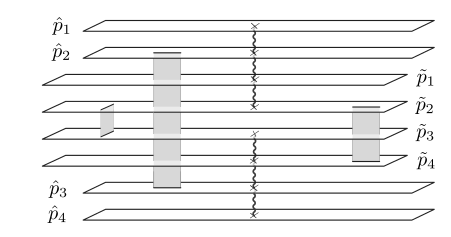
\includegraphics[width=0.75\textwidth]{../graphics/cuts}
	\caption[Example of a classical spectral curve]{Examples of cuts connecting the eight sheets of the Riemann surface corresponding to the classical spectral curve for strings in $AdS_5 \times S^5$. The wavy line corresponds to the pole at $x = 1$.}
	\label{fig:cuts}
\end{figure}

The physical picture is that each cut between two sheets represents an excitation whose polarization is determined by the sheets it connects, an example is shown in figure \ref{fig:cuts}. 
Four of the eight sheets correspond to the $AdS_5$ part of the string target space and the other four to the $S^5$ part. 
$\adsfive$ has $16 = 8_B + 8_F$ types of excitations, in the algebraic curve language this is implemented as a requirement that only sheets from the following sets be connected
\begin{equation}
	\label{eq:polarizations}
	i \in \{ \, \tilde{1}, \, \tilde{2}, \, \hat{1}, \, \hat{2} \, \}, \;\;\;\; j \in \{ \, \tilde{3}, \, \tilde{4}, \, \hat{3}, \, \hat{4} \, \},
\end{equation}
furthermore bosonic excitations correspond to cuts between sheets of the same type (hat or tilde), whereas fermionic excitations connect sheets of different types. 
Obviously fermions do not exist at the classical level, thus cuts can only represent the 8 types of bosonic excitations.
Fermionic excitations start appearing as microscopic cuts, i.e. poles during quantization. 
Solutions in closed sectors, e.g. strings moving in the $\mathbb{R} \times S^3$ submanifold of the target space will be limited to cuts between a subset of the eight sheets.

Denote the branch cut between sheets $i$ and $j$ as $\mathcal{C}^{ij}$, the quasi-momenta on these sheets have discontinuities when going through the cut given by
\begin{equation}
	p_i(x + i\epsilon) - p_j(x - i\epsilon) = 2 \pi n_{ij},
	\label{eq:cut_condition}
\end{equation}  
where $n_{ij}$ is an integer mode number arising due to the logarithm.
For each cut we associate the so called \emph{filling fraction} defined by
\begin{equation}
	\label{eq:filling}
	S_{ij} = \pm \frac{\lambda}{8 \pi^2 i} \oint_{\mathcal{C}^{ij}} \left( 1 - \frac{1}{x^2} \right) p_i(x) dx,
\end{equation}
where the sign is $+1$ for $i=\hat{1},\hat{2}$ and $-1$ for $i=\tilde{1},\tilde{2}$. These are the action variables of the theory \cite{Dorey:2006zj}, roughly they measure the length of the cut and in the physical picture they correspond to the amplitude of the excitation. 
They can be shown to take on integer values, which is natural since we anticipate the classical cuts to be collections of large numbers of poles which condense in the classical limit.
Thus we see that the algebraic curve construction acts like a Fourier decomposition -- string solutions are described as collections of excitations each having definite polarizations, mode numbers and amplitudes.

Let us now review some of the analyticity properties of the quasi-momenta. 
Since the Lax connection has poles at $x = \pm 1$, so do the quasi-momenta (as shown in figure \ref{fig:cuts}). 
Due to the Virasoro constraint, which comes about from the diffeomorphism invariance of the worldsheet, the residues of the quasi-momenta are constrained to
\begin{equation}
	\label{eq:residue_sync}
	\{ \hat{p}_1, \; \hat{p}_2, \; \hat{p}_3, \; \hat{p}_4 \; | \; \tilde{p}_1, \; \tilde{p}_2, \; \tilde{p}_3, \; \tilde{p}_4 \} = \frac{\{ \, \alpha_{\pm}, \, \alpha_{\pm}, \, \beta_{\pm}, \, \beta_{\pm}, \, | \, \alpha_{\pm}, \, \alpha_{\pm}, \, \beta_{\pm}, \, \beta_{\pm} \}}{x \pm 1}.
\end{equation}
An additional constraint on the quasi-momenta comes from the fact that the algebra $\alg{psu}{2,2|4}$ has an automorphism, which is the cause for the $\mathbb{Z}_4$ grading. 
The constraints are given by \cite{Gromov:2008ec}
\begin{eqnarray}
	\label{eq:quasi_inversion}
	\tilde{p}_{1,2}(x) & = & -\tilde{p}_{2,1}(1/x) - 2 \pi m \nonumber \\
	\tilde{p}_{3,4}(x) & = & -\tilde{p}_{4,3}(1/x) + 2 \pi m \nonumber \\
	\hat{p}_{1,2,3,4}(x) & = & -\hat{p}_{2,1,4,3}(1/x).
\end{eqnarray}
These relations define an inversion symmetry $x \rightarrow 1/x$. 
Finally one can look at the asymptotics of the quasi-momenta as the spectral parameter becomes infinite. In this limit the Lax connection becomes related to the Noether currents of the theory and hence one can relate the quasi-momenta to the charges of the global symmetry algebra by \cite{Arutyunov:2004yx,Beisert:2005bm}
\begin{equation}
\left(
\begin{array}{c}
  \hat{p}_1 \\
  \hat{p}_2 \\
  \hat{p}_3 \\
  \hat{p}_4 \\
  \hline
  \tilde{p}_1 \\
  \tilde{p}_2 \\
  \tilde{p}_3 \\
  \tilde{p}_4 \\
\end{array}
\right) = \frac{2 \pi}{x}
\left(
\begin{array}{c}
  + \mathcal{E} - \mathcal{S}_1 + \mathcal{S}_2 \\
  + \mathcal{E} + \mathcal{S}_1 - \mathcal{S}_2 \\
  - \mathcal{E} - \mathcal{S}_1 - \mathcal{S}_2 \\
  - \mathcal{E} + \mathcal{S}_1 + \mathcal{S}_2 \\
  \hline
  + \mathcal{J}_1 + \mathcal{J}_2 - \mathcal{J}_3 \\
  + \mathcal{J}_1 - \mathcal{J}_2 + \mathcal{J}_3 \\
  - \mathcal{J}_1 + \mathcal{J}_2 + \mathcal{J}_3 \\
  - \mathcal{J}_1 - \mathcal{J}_2 - \mathcal{J}_3 \\
\end{array}
\right),
\label{eq:quasi_asymptotics}
\end{equation}
where the charges are rescaled by $\mathcal{Q} = Q / \sqrt{\lambda}$. 
Thus we see that we can characterize the quasi-momenta by describing their behaviour at poles, under symmetries, by their asymptotics and their filling fractions. 

Finally one may ask how this picture of Riemann surfaces with cuts emerges from the gauge theory perspective where the spectrum is described by the Bethe ansatz. 
In the scaling limit when lengths of operators become large the Bethe roots $u_i$ start condensing in the complex plane and start looking like cuts. 
Naturally it is tempting to interpret the cuts of the algebraic curve as collections of very large numbers of poles.
Ultimately a string Bethe ansatz was proposed describing the distribution of these poles \cite{Arutyunov:2004vx},
\beq
	\(\frac{x_j^+}{x_j^-}\)^L = \prod_{j\neq i}^M \frac{u_i - u_j + i}{u_i - u_j - i} \sigma^2_{AFS}(u_i, u_j),
\eeq
where $\sigma_{AFS}$ is the dressing phase.
Compared to the asymptotic Bethe ansatz for the $\alg{su}{2}$ sector
\beq
	\(\frac{x_j^+}{x_j^-}\)^L = \prod_{j\neq i}^M \frac{u_i - u_j + i}{u_i - u_j - i},
\eeq
it is natural to assume that there should be an interpolating Bethe ansatz valid to all orders of the coupling constant.
Indeed the all-loop asymptotic Bethe ansatz for the full superconformal algebra was formulated \cite{Beisert:2005fw} as we described briefly in the previous sections, which interpolated nicely between gauge theory and the algebraic curve. 
In particular the dressing phase $\sigma_{AFS}$ is a limit of the full dressing phase \eq{eq:deformed_dressing} one finds when deforming to long range spin chains.

\subsubsection{Quantization and semi-classics}

Consider a classical string solution characterized by some conserved charges, expanding the superstring action around this solution produces a quadratic lagrangian whose quantization yields the semiclassical spectrum
\beq
	\label{eq:quant_energy_full}
	E(\{N_{ij,n}\}) = E_{cl} + E_0 + \sum_{ij,n} N_{ij,n} \mathcal{E}_{ij,n},
\eeq
where $N_{ij,n}$ is the number of excited quanta with energy $\mathcal{E}_{ij,n}$. Here $ij$ label the different polarizations and $n$ the mode numbers of the excitations. The classical energy is $E_{cl}$ whereas $E_0$ is the ground state energy coming from quantization, the last two terms in \eq{eq:quant_energy_full} are analogues of $\frac{1}{2} \omega$ and $N \omega$ for the harmonic oscillator. Just like in the case of the harmonic oscillator we can infer the ground state energy given the level spacings, it is simply
\beq
	E_0 = \frac{1}{2} \sum_{ij,n}(-1)^{F_{ij}} \mathcal{E}_{ij,n},
\eeq
where $(-1)^{F_{ij}} = \pm 1$ for bosonic/fermionic excitations. In this section we will review the quantization procedure in the algebraic curve formalism \cite{Gromov:2008ec}, which is equivalent to the semi-classical computation of quadratic fluctuations in the sigma-model \cite{Frolov:2002av,Frolov:2003tu,Park:2005ji}, yet is significantly more efficient.

Roughly the idea is that given a classical string solution represented by some cuts between sheets, as seen for example in figure \ref{fig:cuts}, we perturb it by adding microscopic cuts, which can be treated as a finite number of poles.
Just like before the indices $ij$ denoting the connected sheets represent the polarization of the excitation, they can take on values given in \eq{eq:polarizations}, however unlike in the classical setting the excitations can be fermionic as well.
The introduction of these fluctuations backreacts on the classical quasi-momenta $p_k(x)$ shifting them slightly to
\beq
	p_k(x) \rightarrow p_k(x) + \delta^{ij}_n p_k(x).
\eeq
The shifted quasi-momenta still have to satisfy \eq{eq:cut_condition}, which determines the positions $x_n^{ij}$ of the poles
\beq
	\label{eq:pole_pos}
	p_i(x_n^{ij}) - p_j(x_n^{ij}) = 2 \pi \, n_{ij}.
\eeq
The fluctuation will add a pole to the quasi-momentum at this position
\beq
	\delta^{ij}_n p_i = \epsilon_i \frac{\alpha(x^{ij}_n)}{x-x_n^{ij}},
\eeq
where the signs are
\beq
	\epsilon_{\hat{1}} = \epsilon_{\hat{2}} = -\epsilon_{\hat{3}} = -\epsilon_{\hat{4}} = -\epsilon_{\tilde{1}} = -\epsilon_{\tilde{2}} = \epsilon_{\tilde{3}} = \epsilon_{\tilde{4}} = 1
\eeq
and the residue is chosen such that the filling fraction \eq{eq:filling} increases by one, namely
\beq
	\alpha(x) = \frac{4\pi}{\sqrt{\lambda}} \frac{x^2}{x^2 - 1}.
\eeq
The total shifted quasi-momentum is obtained by summing over all fluctuations
\beq
	\delta p_i \sim \sum_{ij} \epsilon_i N_n^{ij} \frac{\alpha(x_n^{ij})}{x-x_n^{ij}}.
\eeq
It still has to satisfy all the analyticity properties outlined in the previous section, this in turn imposes a lot of constraints of the shifts themselves.
The Virasoro constraint implies the synchronization of residues \eq{eq:residue_sync}, which for the shifts translates to
\begin{equation}
	\{ \delta\hat{p}_1, \, \delta\hat{p}_2, \, \delta\hat{p}_3, \, \delta\hat{p}_4 \, | \, \delta\tilde{p}_1, \, \delta\tilde{p}_2, \, \delta\tilde{p}_3, \, \delta\tilde{p}_4 \} = \frac{\{ \, \delta\alpha_{\pm}, \, \delta\alpha_{\pm}, \, \delta\beta_{\pm}, \, \delta\beta_{\pm}, \, | \, \delta\alpha_{\pm}, \, \delta\alpha_{\pm}, \, \delta\beta_{\pm}, \, \delta\beta_{\pm} \}}{x \pm 1}.
\end{equation}
Similarly the asymptotics of the quasi-momenta encode the global charges as seen in \eq{eq:quasi_asymptotics}, for the shifts this translates to
\begin{equation}
\left(
\begin{array}{c}
  \delta \hat{p}_1 \\
  \delta \hat{p}_2 \\
  \delta \hat{p}_3 \\
  \delta \hat{p}_4 \\
  \hline
  \delta \tilde{p}_1 \\
  \delta \tilde{p}_2 \\
  \delta \tilde{p}_3 \\
  \delta \tilde{p}_4 \\
\end{array}
\right) = \frac{4 \pi}{x \sqrt{\lambda}}
\left(
\begin{array}{rl}
  + \delta \Delta/2 &+ N_{\hat{1}\hat{4}} + N_{\hat{1}\hat{3}} + N_{\hat{1}\tilde{3}} + N_{\hat{1}\tilde{4}} \\
  + \delta \Delta/2 &+ N_{\hat{2}\hat{3}} + N_{\hat{2}\hat{4}} + N_{\hat{2}\tilde{4}} + N_{\hat{2}\tilde{3}} \\
  - \delta \Delta/2 &- N_{\hat{2}\hat{3}} - N_{\hat{1}\hat{3}} - N_{\tilde{1}\hat{3}} - N_{\tilde{2}\hat{3}} \\
  - \delta \Delta/2 &- N_{\hat{1}\hat{4}} - N_{\hat{2}\hat{4}} - N_{\tilde{2}\hat{4}} - N_{\tilde{1}\hat{4}} \\
  \hline
   &- N_{\tilde{1}\tilde{4}} - N_{\tilde{1}\tilde{3}} - N_{\tilde{1}\hat{3}} - N_{\tilde{1}\hat{4}} \\
   &- N_{\tilde{2}\tilde{3}} - N_{\tilde{2}\tilde{4}} - N_{\tilde{2}\hat{4}} - N_{\tilde{2}\hat{3}} \\
   &+ N_{\tilde{2}\tilde{3}} + N_{\tilde{1}\tilde{3}} + N_{\hat{1}\tilde{3}} + N_{\hat{2}\tilde{3}} \\
   &+ N_{\tilde{1}\tilde{4}} + N_{\tilde{2}\tilde{4}} + N_{\hat{2}\tilde{4}} + N_{\hat{1}\tilde{4}} \\
\end{array}
\right) + \ord{\frac{1}{x^2}},
\label{eq:quasi_shift_asymptotics}
\end{equation}
where $\delta\Delta$ is the energy shift due to the additional excitations. From here one can read off the individual fluctuation frequencies
\beq
	\label{eq:quasi_energy}
	\Omega_n^{ij} = -2 \delta_{i,\hat{1}} + \frac{\lambda}{2\pi} \lim_{x\rightarrow \infty} x \, \delta_n^{ij} p_{\hat{1}}(x)
\eeq
and the energy shift is then a sum over all frequencies
\beq
	\delta \Delta = \sum_{ij,n} N_{ij}^n \Omega_n^{ij}.
\eeq
The description outlined above is fully sufficient to calculate the semi-classical spectrum around a classical solution -- one has to find the locations of poles, find shifts to the quasi-momenta by utilizing their analyticity properties and finally calculate the 16 fluctuation frequencies and sum them up. 
This produces the energy shift
\beq
\delta \Delta = E(\{N_{ij,n}\}) - E(\{\}) = \sum_{ij,n} N_{ij}^n \Omega_n^{ij},
\eeq
Another quantity of interest is the one-loop shift
\beq
	\label{eq:one_loop_shift}
	E_0 = \frac{1}{2} \sum_{ij,n}(-1)^{F_{ij}} \Omega_n^{ij}
\eeq
appearing in the loop expansion of the energy of a string state as
\beq
	E(\{\}) = E_{cl} + E_0 + \ord{1/\sqrt{\lambda}},
\eeq
where the classical energy $E_{cl}$ is of order $\sqrt{\lambda}$ and $E_0$ is of order $1$.
One can of course proceed with semi-classical quantization, find all the fluctuation frequencies and sum them up by hand to find the one-loop shift, however it would be nicer to find the result in one go.
To that end we introduce the off-shell fluctuations $\delta^{ij} p_k(x;y)$ which are defined by the same asymptotics as the on-shell fluctuations $\delta^{ij}_n p_k(x)$ but the position of the pole is left unspecified, namely
\beq
	\delta^{ij}_n p_k(x) = \delta^{ij} p_k(x;y) \vert_{y=x_n^{ij}}.
\eeq
Note that the off-shell quantity depends on the mode number $n$, which is a function of the pole position via \eq{eq:pole_pos}, which we simply left unspecified as $y$ in the off-shell quantity.
Similarly we introduce off-shell fluctuation energies
\beq
	\Omega_n^{ij} = \Omega^{ij}(y)\vert_{y=x_n^{ij}},
\eeq
which can easily be found if the on-shell frequencies are known by
\beq
	\label{eq:off_shell_freq}
	\Omega^{ij}(y) = \Omega_n^{ij}\vert_{n\rightarrow \frac{p_i(y) - p_j(y)}{2\pi}}.
\eeq
The main advantage of introducing the off-shell frequencies is that due to the $\mathbb{Z}_4$ grading of the $\alg{psu}{2,2|4}$ algebra the quasi-momenta enjoy an inversion symmetry under $x \rightarrow 1/x$ as seen in \eq{eq:quasi_inversion}.
This constrains the off-shell frequencies as well.
Consider symmetric classical configurations that have pairwise symmetric quasi-momenta
\beq
	p_{\hat{1},\hat{2},\tilde{1},\tilde{2}} = -p_{\hat{4},\hat{3},\tilde{4},\tilde{3}},
\eeq
it is known to be the case for all rank one solutions \cite{Gromov:2008ec}, which in particular are dual to states in the $\alg{su}{2}$ and $\alg{sl}{2}$ sectors of $\N=4$ super Yang-Mills. 
All of the off-shell frequencies can then be expressed in terms of two, namely $\Omega^{\tilde2 \tilde3}$ and $\Omega^{\hat2 \hat3}$, which we denote as the basis of frequencies.
The rest of the fluctuations are given by
\beq
\begin{aligned}
\label{eq:freq_relations}
\Omega^{\tilde1\tilde4} (y) &= -  \Omega^{\tilde2 \tilde3}(1/y) +\Omega^{\tilde2\tilde3}(0)\cr 
\Omega^{\tilde2 \tilde4} (y) =
\Omega^{\tilde1\tilde3}(y)  &= {1\over 2} \left( \Omega^{\tilde2 \tilde3}(y) + \Omega^{\tilde1\tilde4} (y) \right)
                               = {1\over 2} \left( \Omega^{\tilde2 \tilde3}(y) - \Omega^{\tilde2\tilde3} (1/y)+\Omega^{\tilde2\tilde3}(0) \right)
                                 \cr
 \Omega^{\hat1\hat4} (y) & = - \Omega^{\hat2 \hat3}(1/y) -2 \cr
\Omega^{\hat2 \hat4} (y) =
\Omega^{\hat1 \hat3} (y) &= {1\over 2}  \left( \Omega^{\hat2 \hat3}(y) + \Omega^{\hat1\hat4} (y) \right)
				    = {1\over 2}  \left( \Omega^{\hat2 \hat3}(y) - \Omega^{\hat2\hat3} (1/y) \right) -1 \cr
\Omega^{\hat2\tilde4}(y) =
\Omega^{\tilde1 \hat3} (y) &= {1\over 2} \left(\Omega^{\hat2 \hat3}(y)+ \Omega^{\tilde1\tilde4} (y)  \right)
				   = {1\over 2} \left( \Omega^{\hat2 \hat3}(y)- \Omega^{\tilde2 \tilde3}(1/y)+\Omega^{\tilde2\tilde3}(0) \right)  \cr				
\Omega^{\tilde2\hat4}(y)=
\Omega^{\hat1 \tilde3} (y) &= {1\over 2} \left( \Omega^{\tilde2\tilde3} (y) + \Omega^{\hat1 \hat4}(y)\right)
				 = {1\over 2}  \left( \Omega^{\tilde2\tilde3} (y) - \Omega^{\hat2 \hat3}(1/y)\right)   -1 \cr
\Omega^{\tilde1 \hat4} (y) =
\Omega^{\hat1 \tilde4} (y) &= {1\over 2} \left( \Omega^{\tilde1 \tilde4}(y) + \Omega^{\hat1\hat4} (y) \right)
				   = {1\over 2} \left(- \Omega^{\tilde2\tilde3}(1/y) - \Omega^{\hat2\hat3}(1/y)+\Omega^{\tilde2\tilde3}(0) \right)
				   -1  \cr	
\Omega^{\hat2\hat3}(y)=
\Omega^{\tilde2 \hat3} (y) &= {1\over 2} \left( \Omega^{\tilde2 \tilde3}(y) + \Omega^{\hat2\hat3} (y) \right)	 \,.
\end{aligned}
\eeq
Knowing the off-shell frequencies and the quasi-momenta one can express the one-loop shift as a contour integral
\beq
	\label{eq:one_loop_integral}
	E_0 = \frac{1}{2} \sum_{ij} (-1)^{F_{ij}} \oint \frac{dx}{2\pi i} \( \Omega^{ij}(x) \d_x \log \sin \frac{p_i - p_j}{2} \),
\eeq
where the integrand is chosen carefully such that it contains poles at each fluctuation insertion point $x_n^{ij}$ with residues $\Omega^{ij}(x_n^{ij})$, so that the result is equivalent to \eq{eq:one_loop_shift}.
There are three contributions to one loop energy shift that are different by their nature.
They can be separated into an ``anomaly" contribution, a contribution from the dressing phase
and a wrapping contribution, which is missing in the asymptotic Bethe ansatz.
\beq
E_0=\delta \Delta_{\rm anomaly} +\delta \Delta_{\rm dressing} + \delta \Delta_{\rm wrapping}\;,
\eeq
where each of these contributions is simply an integral of some closed form expression,
\beqa
\label{eq:delta_E_3}
  \delta \Delta_{\rm anomaly} &=& -\frac{4}{ab-1}\int_a^b \frac{dx} {2\pi i}
  \frac{y(x)}{x^2-1} \partial_x \log \sin p_{\hat 2}\;,\\
  \label{eq:delta_E_1}
  \delta \Delta_{\rm dressing} &=& \sum_{ij} (-1)^{F_{ij}} \int\limits_{-1}^{1} \frac{dz} {2\pi
    i} \left( \Omega^{ij}(z) \, \partial_z \frac{i (p_i -p_j)}{2} \right)\;,\\
  \label{eq:delta_E_2}
  \delta \Delta_{\rm wrapping} &=& \sum_{ij} (-1)^{F_{ij}} \int\limits_{-1}^{1} \frac{dz} {2\pi
    i} \left( \Omega^{ij}(z) \, \partial_z \log (1- e^{-i(p_i -p_j)}) \right)\;.
\eeqa
As always $i$ takes values $\hat 1,\hat 2,\tilde 1,\tilde 2$ whereas $j$ runs over $\hat 3,\hat 4,\tilde 3,\tilde 4$.

\subsubsection{Folded string}
\label{sec:folded_string}

Operators \eq{eq:sl2_operators} from the $\alg{sl}{2}$ sector are known to be dual to folded rotating string solutions in $\adsfive$, these are closed strings rotating around their center of mass in an $AdS_3$ subspace of $AdS_5$ with spin $S$ \cite{Frolov:2002av}.
Additionally they orbit the big circle of $S^5$ with angular momentum $J$, also referred to as twist.
These parameters as expected correspond to the number of scalars $J$ and number of derivatives $S$ in the gauge theory operators. 
In the classical regime these are assumed to scale as $\sqrt{\lambda}$, thus we use $\mathcal{S} = S/ n \sqrt{\lambda}$ and $\mathcal{J} = J / n \sqrt{\lambda}$ when describing the classical solution, which corresponds to long operators in gauge theory. 
The number of spikes $n$ corresponds to the mode number $n$ in the language of Bethe states.

Given the explicit string solution (see \cite{Tseytlin:2010jv} for details) one could follow the steps outlined in the classical spectral curve construction, namely calculate the monodromy matrix \eq{eq:monodromy}, diagonalize it and extract the quasi-momenta. 
While it is indeed possible to do, we will present an alternative method based on analyticity properties of the quasi-momenta when we discuss the classical limit of cusped Wilson lines in section \ref{sec:wilson_classical}.
Here we present the result \cite{Gromov:2011de}, which consists of two ``basis'' quasi-momenta
\beqa
  \label{eq:p_a}\nn
  p_{\hat 2} &=& \pi n - 2\pi n{\cal J} \left( \frac{a}{a^2-1} -
    \frac{x}{x^2-1} \right) \sqrt{\frac{(a^2-1)
      (b^2-x^2)}{(b^2-1)(a^2-x^2)}} \\ \nn &+& \frac{8\pi\, n\, a b\, {\cal S} F_1(x)}{(b-a)(ab+1)} +
  \frac{2\pi n {\cal J} (a-b) F_2(x)}{\sqrt{(a^2-1)(b^2-1)}},\\
  \label{eq:p_s}
  p_{\tilde 2} &=& \frac{2\pi {\cal J}x}{x^2-1},
\eeqa
while the remaining functions can be determined by utilizing the $x \rightarrow 1/x$ inversion symmetry as shown in \eq{eq:quasi_inversion}, resulting in
\beqa
  \label{eq:quasi-momenta_symmetry_A}
  p_{\hat{2}} (x) &=& -p_{\hat{3}}(x) = -p_{\hat{1}}(1/x) = p_{\hat{4}}
  (1/x)\;,\\
  \label{eq:quasi-momenta_symmetry_S}
  p_{\tilde{2}} (x) &=& -p_{\tilde{3}} (x) = p_{\tilde{1}} (x) =
  -p_{\tilde{4}}(x)\;.
\eeqa
The functions $F_1(x)$ and $F_2(x)$ can be expressed
in terms of the elliptic integrals:
\begin{eqnarray}
 \label{eq:not}
 F_1(x) &=& i F \left( i \sinh^{-1}
 \left. \sqrt{\frac{(b-a)(a-x)}{(b+a)(a+x)}} \right\vert\frac{(a+b)^2}{(a-b)^2} \nonumber
 \right)\;, \\
\nn
 F_2(x) &=& i E \left( i \sinh^{-1}
 \left.\sqrt{\frac{(b-a)(a-x)}{(b+a)(a+x)}} \right\vert \frac{(a+b)^2}{(a-b)^2}
 \right)\;.
 \end{eqnarray}
This is a two-cut solution with symmetric cuts on the real axis given by the branch points $a < b$ (and $-b < -a$).
 The classical energy $\Delta$ of the folded string is a function of the Lorentz spin $\mathcal{S}$,
twist $\mathcal{J}$ and the mode number $n$. This function can be written in a parametric form
in terms of the branch points $a$ and $b$ \cite{Gromov:2011de,Beisert:2003ea,Kazakov:2004qf,Kazakov:2004nh}:
\beqa
\nn{2\pi {\cal S}}&=&\frac{ab+1}{ab}\[b E\(1-\tfrac{a^2}{b^2}\)-aK\(1-\frac{a^2}{b^2}\)\]\;,\\
{2\pi {\cal J}}&=&\frac{2\sqrt{(a^2-1)(b^2-1)}}{b}K\(1-\frac{a^2}{b^2}\)\;,\\
\nn{2\pi {\cal D}}&=&\frac{ab-1}{ab}\[b E\(1-\tfrac{a^2}{b^2}\)+aK\(1-\frac{a^2}{b^2}\)\]\;.
\eeqa
where ${\cal D}=\Delta / n\sqrt\lambda$ and $E$, $K$ are elliptic integrals of the first kind.

Next we proceed to the semi-classical quantization of the folded string solution, more precisely we are after the one-loop shift.
Instead of calculating the 16 fluctuation frequencies $\Omega_n^{ij}$ we adopt the off-shell frequency formalism outlined above.
Once again, the exact formulae for the off-shell frequencies can be found solely from analyticity constraints by first determining the off-shell shifts in quasi-momenta and then using the definitions \eq{eq:quasi_energy} and \eq{eq:off_shell_freq}.
The answer turns out to be surprisingly simple and is given by the two basis frequencies
\beqa
\label{oma}
\Omega^{\tilde 2\tilde 3}(x)&=&\frac{2}{a
  b-1}\frac{\sqrt{a^2-1}\sqrt{b^2-1}}{x^2-1}\;,\\
\label{oms}
\Omega^{\hat 2\hat 3}(x)&=&\frac{2}{a b-1}\(1-\frac{y(x)}{x^2-1}\)\;.
\eeqa
where $y(x)=\sqrt{x-a} \sqrt{a+x} \sqrt{x-b} \sqrt{b+x}$.
The remaining frequencies can be read off from the relations \eq{eq:freq_relations}.
What remains in order to find the one-loop shift is performing the sum \eq{eq:one_loop_shift} or alternatively evaluating the integral \eq{eq:one_loop_integral} numerically.
The answer involves an infinite sum over all mode numbers hence it is not very illuminating at this point.

Let us now consider the $\mathcal{S} \rightarrow 0$ limit.
The square of the classical energy has a very nice expansion in this limit
\beqa
	\label{eq:classical_energy}
 {\cal D}^2&=&{\cal J}^2+2 \, {\cal S} \, \sqrt{{\cal J}^2+1}+{\cal S}^2 \, \frac{2 {\cal J}^2+3}{2
   {\cal J}^2+2}-{\cal S}^3 \, \frac{{\cal J}^2+3}{8
   \left({\cal J}^2+1\right)^{5/2}}
   %+{\cal S}^4\frac{3 {\cal J}^4+18 {\cal J}^2+31}{64 \left({\cal J}^2+1\right)^4}
   +{\cal O}\left({\cal S}^4\right)\;.\qquad
\eeqa
The one-loop shift expanded up to two orders in $\mathcal{S}$ reads
\small
\beqa
\label{eq:delta_oneloop_slope}
\Delta&\simeq&
\frac{-{\cal S}}{2 \left({\cal J}^3+{\cal J}\right)}+{\cal S}^2\[\frac{3 {\cal J}^4+11 {\cal J}^2+17
   }{16 {\cal J}^3 \left({\cal J}^2+1\right)^{5/2}}
\!-\!\sum_{\substack{m>0 \\ m \neq n}}\frac{n^3m^2  \left(2 m^2+n^2 {\cal J}^2-n^2\right)}{{\cal J}^3 \left(m^2-n^2\right)^2
   \left(m^2+n^2 {\cal J}^2\right)^{3/2}}\]. \;\;\;\;\;\;\;\;
   \;.
\eeqa
\normalsize
%The next terms in this expansion can be found in \eq{delta_oneloop_3}, \eq{delta_oneloop_4}. 
The sum is nothing but a sum over the fluctuation energies,
whereas the remaining terms originate from the ``zero"-modes
$m=n$, which have to be treated separately.
The sum can be very easily expanded for small ${\cal J}$.
It is easy to see that the expansion coefficients will be certain combinations
of zeta-functions. It is also easy to see that
the dependence on the mode number $n$ is rather nontrivial.
The expansion of the one loop energy first in small ${\cal S}$
up to a second order and then in small ${\cal J}$ reads
\beq
\label{delta_oneloop_sj}
\Delta_{\rm1-loop}\simeq
\left\{
\begin{array}{ll}
 -\frac{\mathcal{S}}{2 \mathcal{J}}+
 \mathcal{S}^2 \left(+\frac{1}{2\mathcal{J}^3}-\frac{3 \zeta_3}{2 \mathcal{J}}-\frac{1}{16 \mathcal{J}}\right) & \;\;\;\;\mathrm{for}\;n=1, \\
 -\frac{\mathcal{S}}{2 \mathcal{J}}+
 \mathcal{S}^2 \left(+\frac{1}{2
   \mathcal{J}^3}-\frac{12 \zeta_3}{\mathcal{J}}-\frac{17}{16 \mathcal{J}}\right) & \;\;\;\;\mathrm{for}\; n=2, \\
 -\frac{\mathcal{S}}{2 \mathcal{J}}+
 \mathcal{S}^2 \left(-\frac{5}{8
   \mathcal{J}^3}-\frac{81 \zeta_3}{2 \mathcal{J}}-\frac{7}{4 \mathcal{J}}\right) & \;\;\;\;\mathrm{for}\;n=3. %\\
% -\frac{\mathcal{S}}{2 \mathcal{J}}+
% \mathcal{S}^2 \left(-\frac{55}{18
%   \mathcal{J}^3}-\frac{96 \zeta_3}{\mathcal{J}}-\frac{281}{144 \mathcal{J}}\right) & \;\;,\;\;n=4
\end{array}
\right.
\eeq
%Expansions up to four orders in $\mathcal{S}$ and then in $\mathcal{J}$ are given in appendix \ref{AppS4}. 
We note that the contributions ${\cal S}^2/{\cal J}^3$ are universal for $n=1$ and $n=2$, however starting from $n=3$ we get different coefficients.
%As we will discuss in the next section this could imply that the naive generalization of the conjecture in \cite{Basso:2011rs} is not fully correct for $n>2$. Also for $n=2$ we found  a similar anomaly at the order $S^3$.

\subsection{Short strings}
\label{sec:short_strings}

Even though semi-classical results are technically only valid for the charges scaling as $\sqrt{\lambda}$, there is evidence that re-expanding the classical energy plus the one-loop shift yields a reasonable result in terms of the unscaled charges $J$ and $S$ \cite{Roiban:2009aa}, thus providing one the possibility to probe so-called short string states, the Konishi operator being a prime example.
Namely summing up the square root of \eq{eq:classical_energy} and \eq{delta_oneloop_sj}, introducing the unscaled charges $S = \sqrt{\mu}\, \mathcal{S}$, $J = \sqrt{\mu}\, \mathcal{J}$ and re-expanding in terms of $\mu \equiv n^2 \lambda$ yields the following one-loop energy for the folded string solution \cite{Gromov:2011de}
\beq
\Delta_{S,J,n}\simeq\sqrt{2S}\mu^{1/4}
+\frac{2J^2+3S^2-2S}{4\,(2 S)^{1/2}\,\mu^{1/4}}.
\eeq
For the Konishi operator we get
\beq
\Delta_{2,2,1}=2 \, \lambda^{1/4} + \frac{2}{\lambda^{1/4}}+ \ord{\lambda^{-3/4}},
\eeq
where the first coefficient of the expansion was first derived in \cite{Gubser:2002tv}.
The sub-leading coefficient was first suggested to be $1$ in \cite{Roiban:2009aa}, however a possible issue with the argument was soon pointed out in \cite{Arutyunov:2009ax}, where numerical calculations indeed confirmed the correct answer to be $2$.

In this section we will show how combining the knowledge of the semi-classical one-loop shift \eq{eq:delta_oneloop_slope} and the slope function \eq{eq:slope_function} can yield further information about the Konishi anomalous dimension.
Later in the text when we find the next small spin coefficient after the slope, which we call the curvature function, we will revisit the techniques presented here in order to boost the obtain results one order further.

\subsubsection{Structure of small spin expansions}
\label{sec:small_spin_structure}

Consider the classical string energy \eq{eq:classical_energy}, the re-expansion of $\Delta^2$ in the large $\mu \equiv \lambda n^2$ limit with $S$ and $J$ fixed has a particularly nice structure
\small
\beq
\Delta^2=J^2+S
\(
2\, \sqrt{\mu}+\frac{J^2}{\sqrt{\mu}}+\dots%-\frac{J^4}{4\mu^{3/2}}
\)
+S^2
\(
\frac{3}{2}-\frac{J^2}{2\sqrt{\mu}}
+\dots%+\frac{J^4}{2\mu^2}
\)
-S^3
\(
\frac{3}{8\sqrt{\mu}}
-\frac{13 J^2}{16\sqrt[3]{\mu}}
+\dots
\)
%+S^4\(\frac{31}{64\mu}+\dots\)
+{\cal O}({ S}^4)
\label{dsquare_tree}
\eeq
\normalsize
where each next term in $S$ gets more and more suppressed for large $\mu$. 
It was conjectured \cite{Basso:2011rs} that a generalization of this result holds for any operator at all values of the coupling constant, more precisely the statement was that making expansions of the scaling dimension squared first in $S\to 0$ and then in $\mu\to \infty$ should reveal the following structure
\small
\beq\label{eq:delta_squared_basso}
\Delta^2=J^2+S
\(
A_1\sqrt{\mu}+A_2+\dots
\)
+S^2
\(
B_1+\frac{B_2}{\sqrt\mu}
+\dots%+\frac{J^4}{2\mu^2}
\)
+S^3
\(
\frac{C_1}{\mu^{1/2}}
+\frac{C_2}{\mu^{3/2}}
+\dots
\)
%+S^4\(\frac{31}{64\mu}+\dots\)
+{\cal O}({ S}^4)\;,
\eeq
\normalsize
where the coefficients $A_i,\;B_i,\;C_i$, etc. are some functions of $J$.

\begin{figure}[t]
    \begin{tabular}{cc}
    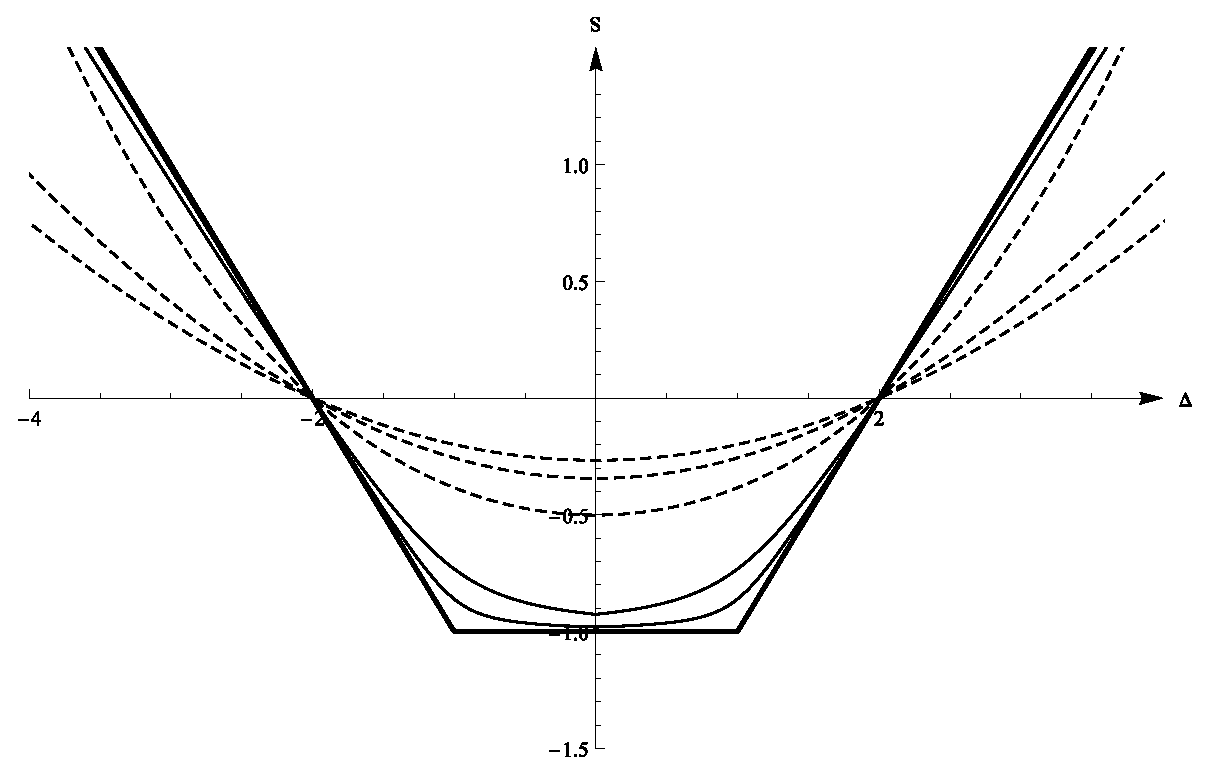
\includegraphics[scale=0.7]{../graphics/bfkl}
    \end{tabular}
\caption[The BFKL trajectories $S(\Delta)$ for the twist-2 operator]{The BFKL trajectories $S(\Delta)$ for the twist-2 operator at various values of the coupling. Solid black lines are obtained using the known two loop weak coupling expansion \cite{Brower:2006ea,Kotikov:2002ab} and dashed lines are obtained using the strong coupling expansion \cite{Costa:2012cb,Kotikov:2013xu,Brower:2013jga}.}
\label{fig:bfkl}
\end{figure}

Indeed it is not hard to understand this constraint.
A good entry point is considering the inverse relation $S(\Delta)$, frequently encountered in the context of BFKL \cite{bfkl,Alfimov:2014bwa}, where one also usually sets $n=1$. 
It satisfies a few basic properties, namely the curve $S(\Delta)$ goes through the points $(\pm J, 0)$ at any coupling, because at $S=0$ the operator is BPS. 
At the same time for non-BPS states one should have $\Delta(\lambda)\propto \lambda^{1/4}\to\infty$ \cite{Gubser:1998bc} which indicates that if $\Delta$ is fixed, $S$ should go to zero, thus combining this with the knowledge of fixed points $(\pm J, 0)$ we conclude that at infinite coupling $S(\Delta)$ is simply the line $S = 0$. 
As the coupling becomes finite $S(\Delta)$ starts bending from the $S=0$ line and starts looking like a parabola going through the points $\pm J$, as shown in figure~\ref{fig:bfkl}. 
Based on this qualitative picture and the scaling $\Delta(\lambda)\propto \lambda^{1/4}$ at $\lambda\rightarrow\infty$ and fixed $J$ and $S$, one can write down the following ansatz,
\beqa
\label{eq:sofdelta}
	S(\Delta) &=& \left( \Delta^2 - J^2\right)\Bigl( \alpha_1 \frac{1}{\lambda^{1/2}} + \alpha_2 \frac{1}{\lambda} + (\alpha_3 + \beta_3 \Delta^2) \frac{1}{\lambda^{3/2}} + (\alpha_4 + \beta_4 \Delta^2) \frac{1}{\lambda^{2}}    \Bigr. \nn\\
	&+&
	\Bigl.
	(\alpha_5 + \beta_5 \Delta^2+\gamma_5\Delta^4) \frac{1}{\lambda^{5/2}}
	+(\alpha_6 + \beta_6 \Delta^2+\gamma_6\Delta^4) \frac{1}{\lambda^{3}}
	+\dots
	\Bigr).
\eeqa
The reason for omitting odd powers of the scaling dimension from the ansatz will become clear later when we discuss the $\pmu$-system, where we will see that only the square of $\Delta$ enters the equations. 
We can now invert the relation and express $\Delta$ in terms of $S$ at strong coupling, which exactly reproduces \eq{eq:delta_squared_basso}. There exists a one-to-one mapping between the coefficients $\alpha_i$, $\beta_i$, etc. and $A_i$, $B_i$ etc, which is rather complicated but easy to find.
% We note that this structure of $\Delta^2$ coincides with Basso's conjecture in \cite{Basso:2011rs} for mode number $n=1$ \footnote{The generalization of \eq{eq:delta_squared_basso} for $n>1$ is not fully clear, as noted in \cite{Gromov:2011bz}, and this case will be discussed in appendix \ref{sec:appN}.}. 
The pattern in \eq{eq:delta_squared_basso} continues to higher orders in $S$ with further coefficients $D_i$, $E_i$, etc. and powers of $\mu$ suppressed incrementally. This structure is a non-trivial constraint on $\Delta$ itself as one easily finds from \eq{eq:delta_squared_basso} that
\small
\beqa\label{eq:delta_small_s}
\Delta&\simeq&J+\frac{S}{2J}
\(
A_1\sqrt{\mu}+A_2+\frac{A_3}{\sqrt{\mu}}+\dots
\)\\
\nn&+&S^2
\(
- \frac{A_1^2}{8J^3} \, \mu
-  \frac{A_1A_2}{4J^3} \, \sqrt{\mu}
+\[\frac{B_1}{2J}-\frac{A_2^2+2A_1 A_3}{8J^3}\]
+
\[
\frac{B_2}{2J}
-\frac{A_2A_3+A_1A_4}{4J^3}
\]  \frac{1}{\sqrt\mu}
+\dots
\),
%+{\cal O}(S^3)\;.
\eeqa
\normalsize
where we introduced the mode number by the naive replacement $\lambda \to \mu \equiv n^2 \lambda$.
By definition the coefficients of $S$ and $S^2$ are the slope and curvature functions respectively as defined in \eq{eq:slope_definition}, so now we have their expansions at strong coupling in terms of $A_i,\;B_i,\;C_i$, etc. 
Since the $S$ coefficient only contains the constants $A_i$, we can find all of their values by simply expanding the slope function \eq{eq:slope_function} that we found earlier at strong coupling. 
We get
\beq
\label{eq:bassos_as}
A_1=2\;\;,\;\;
A_2=-1\;\;,\;\;
A_3=J^2-\frac{1}{4}\;\;,\;\;
A_4=J^2-\frac{1}{4}\dots\;.
\eeq
Note that in this series the power of $J$ increases by two at every other member, which is a direct consequence of omitting odd powers of $\Delta$ from \eq{eq:sofdelta}. 
We also expect the same pattern to hold for the coefficients $B_i$, $C_i$, etc.
It is not hard to see that the sub-leading coefficient in the spin $S$ only contains $A_i$ and $B_i$ coefficients, thus given the $A$'s we could in principle fix all $B$'s.
Hence we conclude that the letters in $A_i$, $B_i$, $C_i$ etc. are directly linked to the generalizations of the slope function $\gamma^{(n)}$.

\subsubsection{Two-loop prediction}

Let us now consider the case $n=1$.
We are interested in the coefficients of the strong coupling expansion of $\Delta$, namely
\beq
	\Delta = \Delta^{(0)} \lambda^\frac{1}{4} + \Delta^{(1)} \lambda^{-\frac{1}{4}}  + \Delta^{(2)} \lambda^{-\frac{3}{4}} + \Delta^{(3)} \lambda^{-\frac{5}{4}} + \dots
\eeq
First, we utilize the structure \eq{eq:delta_squared_basso} and by fixing $S$ and $J$ we re-expand the square root of $\Delta^2$ at strong coupling to find
\beq
	\label{eq:delta_abc}
	\Delta = \sqrt{A_1 S} \, \sqrt[4]{\lambda}  + \frac{\sqrt{A_1} \left( J^2 + A_2 S + B_1 S^2 \right)}{2 A_1 \sqrt{S}} \, \frac{1}{\sqrt[4]{\lambda}} + {\cal O}\(\frac{1}{\lambda^\frac{3}{4}}\).
\eeq
Thus we reformulate the problem entirely in terms of the coefficients $A_i$, $B_i$, $C_i$, etc. For example, the next coefficient in the series, namely the two-loop term is given by
\beq
	\label{eq:delta_2loops_abc}
	\Delta^{(2)} = -\frac{\left(2 A_2 + 4 B_1+J^2\right)^2-16 A_1 (A_3+2 B_2+4 C_1)}{16 \sqrt{2} A_2^{3/2}}.
\eeq
Further coefficients become more and more complicated, however a very clear pattern can be noticed after looking at these expressions: we see that the term $\Delta^{(n)}$ only contains coefficients with indices up to $n+1$, e.g. the tree level term $\Delta^{(0)}$  only depends on $A_1$, the one-loop term depends on $A_1$, $A_2$, $B_1$, etc. Thus we can associate the index of these coefficients with the loop level. Conversely, from the last section we learned that the letter of $A_i$, $B_i$, etc. can be associated with the order in $S$, i.e. the slope function fixed all $A_i$ coefficients and the curvature function in principle fixes all $B_i$ coefficients.

Looking at \eq{eq:delta_abc} we see that knowing $A_i$ and $B_i$ only takes us to one loop, in order to proceed we need to know some coefficients in the $C_i$ and $D_i$ series. This is where the knowledge of the classical energy \eq{eq:classical_energy} and its semi-classical correction \eq{eq:delta_oneloop_slope} come in handy. We add up the classical and the 1-loop contributions, take $S$ and $J$ fixed at strong coupling and compare the result to \eq{eq:delta_squared_basso}. By requiring consistency we are able to extract the following coefficients for $n=1$,
\beqa
 \label{eq:abcd2}
 \begin{array}{rcrlrlrcl}
  A_1 &=&  &2, &A_2&  &=& -&1  \\
  B_1 &=&  &3/2, &B_2&  &=& -&3\,\zeta_3+\frac{3}{8}  \\
  C_1 &=& -&3/8, &C_2& &=& &\frac{1}{16} \, (60 \, \zeta_3 + 60 \, \zeta_5 - 17) \\
  D_1 &=&  &31/64, &D_2& &=& & \frac{1}{512} (-5520 \, \zeta_3 - 5120 \, \zeta_5 -3640 \, \zeta_7 +901). 
 \end{array}
\eeqa
As discussed in the previous section, we can in principle extract all coefficients with indices $1$ and $2$. In order to find e.g. $B_3$ we would need to extend the quantization of the classical solution to the next order. 
% We can now take the small spin expansion of the scaling dimension \eq{eq:delta_small_s} and re-expand it at strong coupling.
% Together with our knowledge of the coefficients $A_i$ coming from the slope function we find
% \beq
% \Delta_{S,J,n}\simeq\sqrt{2S}\mu^{1/4}
% +\frac{2J^2+3S^2-2S}{4\,(2 S)^{1/2}\,\mu^{1/4}}
% +\frac{-21S^4+(32B_2+12)S^3+(20J^2-12)S^2+8J^2 S-4J^4}{32\,(2S)^{3/2}\,\mu^{3/4}}\;.
% \eeq
For general mode numbers $n$ one can extract the following values for $B_i$,
\beq\label{BB}
B_1=\frac{3}{2}\;\;,\;\;
B_2=
\left\{
\bea{ll}
-3\,\zeta_3+\frac{3}{8}&\;\;,\;\;n=1\\
-24\,\zeta_3-\frac{13}{8}&\;\;,\;\;n=2\\
-81\,\zeta_3-\frac{24}{8}&\;\;,\;\;n=3
\eea
\right..\vspace{10pt}
\eeq
Combining all of this information we find the following result for spin 2 operators
\beq
\Delta_{2,J,1}=2 \, \lambda^{1/4}+
\frac{\frac{J^2}{4}+1}{\lambda^{1/4}}+\frac{-\frac{J^4}{64}+\frac{3 J^2}{8}-3\, \zeta
   (3)-\frac{3}{4}}{\lambda^{3/4}} + \ord{\frac{1}{\lambda^{5/4}}}\;,
\eeq
which for Konishi reads
\beq
\Delta_{2,2,1}=2 \, \lambda^{1/4}+
\frac{2}{\lambda^{1/4}}+\frac{\frac{1}{2} -3\, \zeta_3}{\lambda^{3/4}} + \ord{\frac{1}{\lambda^{5/4}}}\;.
\eeq
Generalizing the discussion above we conclude that this procedure yields the $n$-loop scaling dimension given the values of 
\beq
	A_{1,2,\dots,n+1}, \;\;\; B_{1,2,\dots,n}, \;\;\; C_{1,2,\dots,n-1}, \;\;\; \dots, \;\;\; A^{(n+1)}_1,
\eeq
thus e.g. to go to three loops we would need to know $A_{1,2,3,4}$, $B_{1,2,3}$, $C_{1,2}$, $D_1$, where the only unknown at this point is $B_3$.
In order to find it we would either need to find the curvature function $\gamma^{(2)}$ or quantize the classical string to one more order.

\subsubsection{Inconsistencies for higher mode numbers}
\label{sec:inconsistencies}

%Note that according to our observations there are some inconsistencies in the conjecture that this derivation relies on when $n>1$ and thus this result should be treated with great care.\footnote{We assume that the results of \cite{Basso:2011rs} for the slope function
%can be lifted by generalizing with the simple replacement $\lambda\to n^2\lambda$ when $n>1$. 
%We indeed verified this numerically with high precision at weak coupling up to two loops and this is also in agreement
%with our one loop strong coupling results. I.e. the slope function and hence the coefficients $A_i$ in \eq{As} are still correct after the replacement, but as argued before, the structure of the expansion \eq{Delta} may need to be modified.}
%These cases, however, were not analyzed as thoroughly
%as the $n=1$ case in \cite{Basso:2011rs} where some additional tests at weak coupling were made.


%Comparing with our one-loop result we get\footnote{$B_2=-b$ in the notations of \cite{Basso:2011rs}.
%The $-3\zeta_3$ term also arises in the formalism of \cite{Vallilo:2011fj} when formally extended to two loops.
%A very similar $\zeta_3$ term can be also extracted from \cite{Roiban:2011fe}.
%This gives extra support to our results.
%We would like to thank L.Mazzucato and A.Tseytlin for pointing this out.
%}



% We should, however, notice that for $n>1$ we were not able to fully satisfy \eq{cons}.
% One example is the coefficient in front of $S^2/J^3$, which for $n=3$ is $-5/8$, whereas \eq{cons} predicts $1/2$. We observe that only for $S^2$, $S^3$ and higher order terms do we find such disagreements and it is interesting to note that the coefficients for $S$ order terms seem to be correct for any $n$\footnote{We indeed verified numerically that the naive replacement $\lambda\to n^2\lambda$ works at weak coupling at least to two loops.}.
% These observations imply that the generalization of the original slope function,
% which is done by a naive replacement $\lambda\to n^2\lambda$, is not correct for the cases when $n>1$ and thus either the coefficients in \eq{As} or the conjecture itself should be modified to accommodate this.
% We discuss this in details in the next section \ref{inconsistencies}.


The analysis in the previous sections was done only up to second order in the small spin expansion, namely using the one-loop semi-classical energy given by \eq{delta_oneloop_sj}. 
%The appendix \ref{AppS4} contains our result for the one-loop quantization of the $n$-times folded string up to the order $S^4$. 
Extending our results to higher orders in the spin we found perfect agreement with the conjectured structure \eq{eq:delta_squared_basso} for mode number $n=1$, yet for cases with $n>1$ there are inconsistencies.
For $n=2$ the first inconsistency appears in the $\frac{S^3\mu}{J^4}$ term and for $n=3$ there are already inconsistencies at order $S^2$. We found that for $n>1$ one has to modify the structure in \eq{eq:delta_squared_basso} by
including negative coefficients in order for it to be consistent with our one-loop results. E.g. for $n=2$ the structure has to be modified starting with the $S^3$ term, which now becomes
\beq
\(
C_{-2}\;\mu+\frac{C_1}{\sqrt\mu}+\frac{C_2}{\mu}+\dots
\) S^3
\eeq
with $C_{-2}=12/J^4$. To the next order in $S$ we find
\beq
\(
D_{-4}\;\mu^{3/2} +D_{-2}\;\sqrt{\mu}+ \frac{D_{0}}{\sqrt\mu}+\frac{D_1}{\mu}+\dots
\) S^4
\eeq
where $D_{-4}=-\frac{78}{J^6},\;D_{-2}=-\frac{36}{J^4},\;D_0=\frac{21}{2J^2}$.
For $n=3$ the first modification already occurs at order $S^2$ and it can be resolved if the term $-\frac{9 S^2\sqrt\mu}{4 J^2}$ is added to \eq{eq:delta_squared_basso}.
Thus effectively the conjectured structure \eq{eq:delta_squared_basso} has to be modified as in the $n=2$ case by including negative coefficients, which now depend on $n$ in a non-trivial way.
It is also worth noticing that since inconsistencies start appearing at orders of $\frac{S^2}{J^2}$ and $\frac{S^3}{J^4}$ for $n=3$ and $n=2$ respectively, one might guess that
there should be an inconsistency at order $\frac{S^4}{J^6}$ for $n=1$, however we found no such thing.
% This study of inconsistencies reveals that the proposed modifications to the structure of \eq{eq:delta_squared_basso} have growing powers of $\mu$,
% thus one should resum them together with similar singular terms which may arise in higher loop levels before being able to make justified predictions
% for short operators ($S\sim J\sim 1$) at strong coupling when $n>1$.

We will revisit this topic in section \ref{sec:curvature_inconsistencies} when we try to perform this procedure again after having found the curvature function.
As one might expect, similar issues appear in that case as well.



% \subsection{Towards the full solution}

% Mention nested BAE, full psu(2,2|4) spin chain without going into much detail.
